\renewcommand{\figurename}{Diagram}
\subsection{Merge Tracking}

Subversion supports per-directory and per-file merge tracking. The implementation of per-branch merges built on top of per-directory merges. Git tracks per-branch merges only. Hence Translator is able to translate branch-level merges only. In this section we consider common merge scenarios and describe the behavior of Translator for every of them.

\subsubsection{Merge History Basics}

Subversion keeps the history of merges performed on certain branch. It is represented as svn:mergeinfo property set on branch root directory. When Git user performs merge from branch2 to branch1, all commits of branch2 becomes the history of branch1. From Subversion perspective that means that branch1 got branch2 as merge history, i.e. svn:mergeinfo property should include revisions mapped to merged commits. This idea illustrated on diagrams \ref{simple_merge_git_to_svn} and \ref{simple_merge_branch_no_parent_git_to_svn}.

\begin{center}
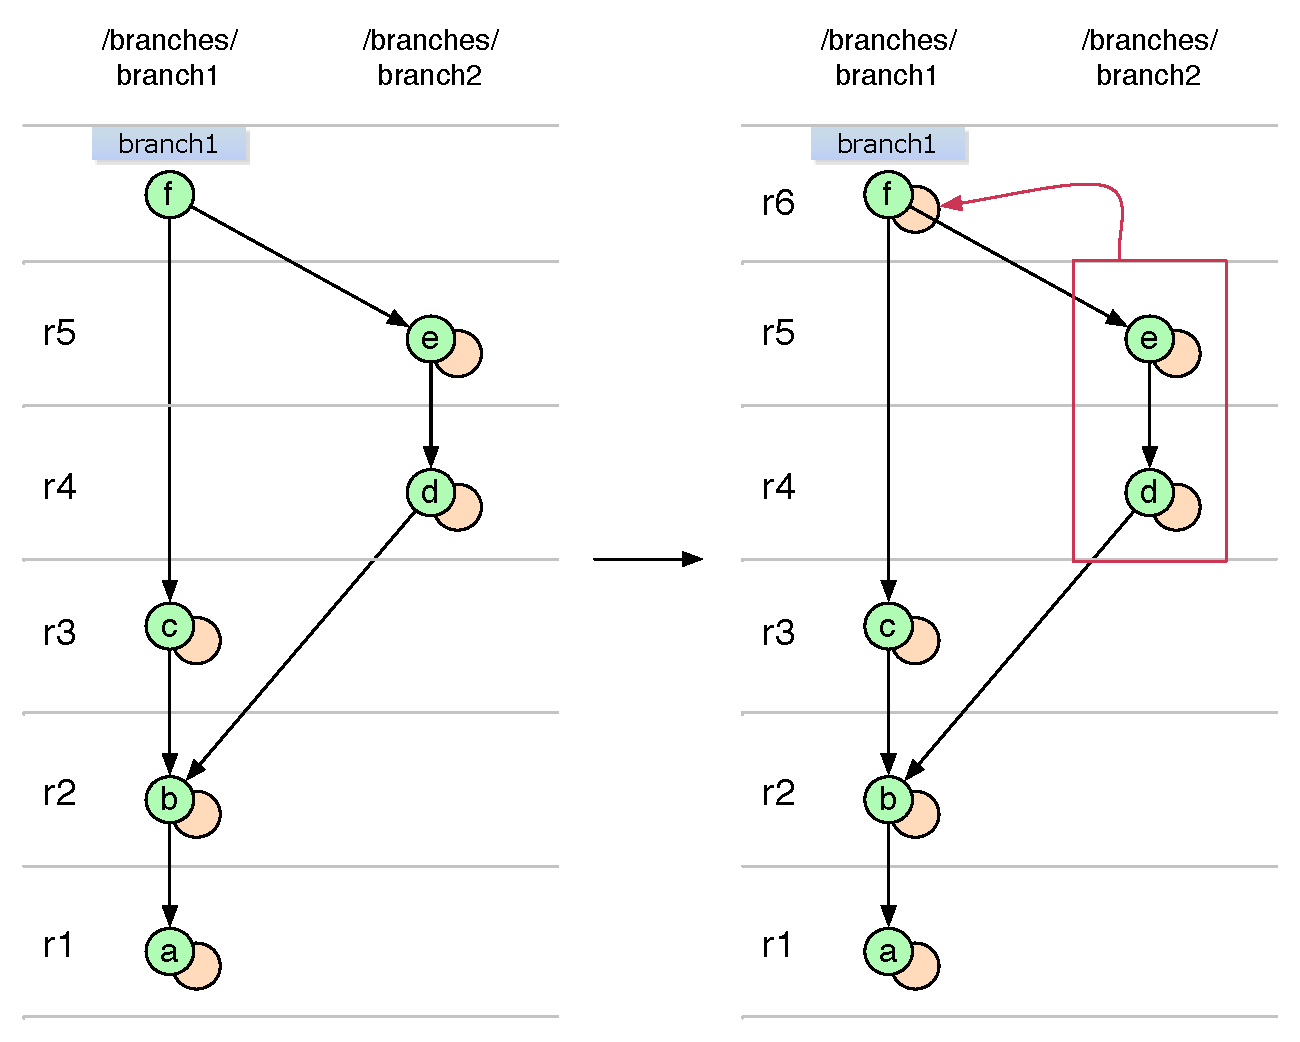
\includegraphics[width=\textwidth]{img/diagrams/simple_merge_git_to_svn.pdf}%
\captionof{figure}{Git merge commit being translated to the change of svn:mergeinfo property.}
\label{simple_merge_git_to_svn}%
\end{center}

The difference between these scenarios is that merged branch2 branch may have common commits with branch1 or no common commits at all.

\begin{center}
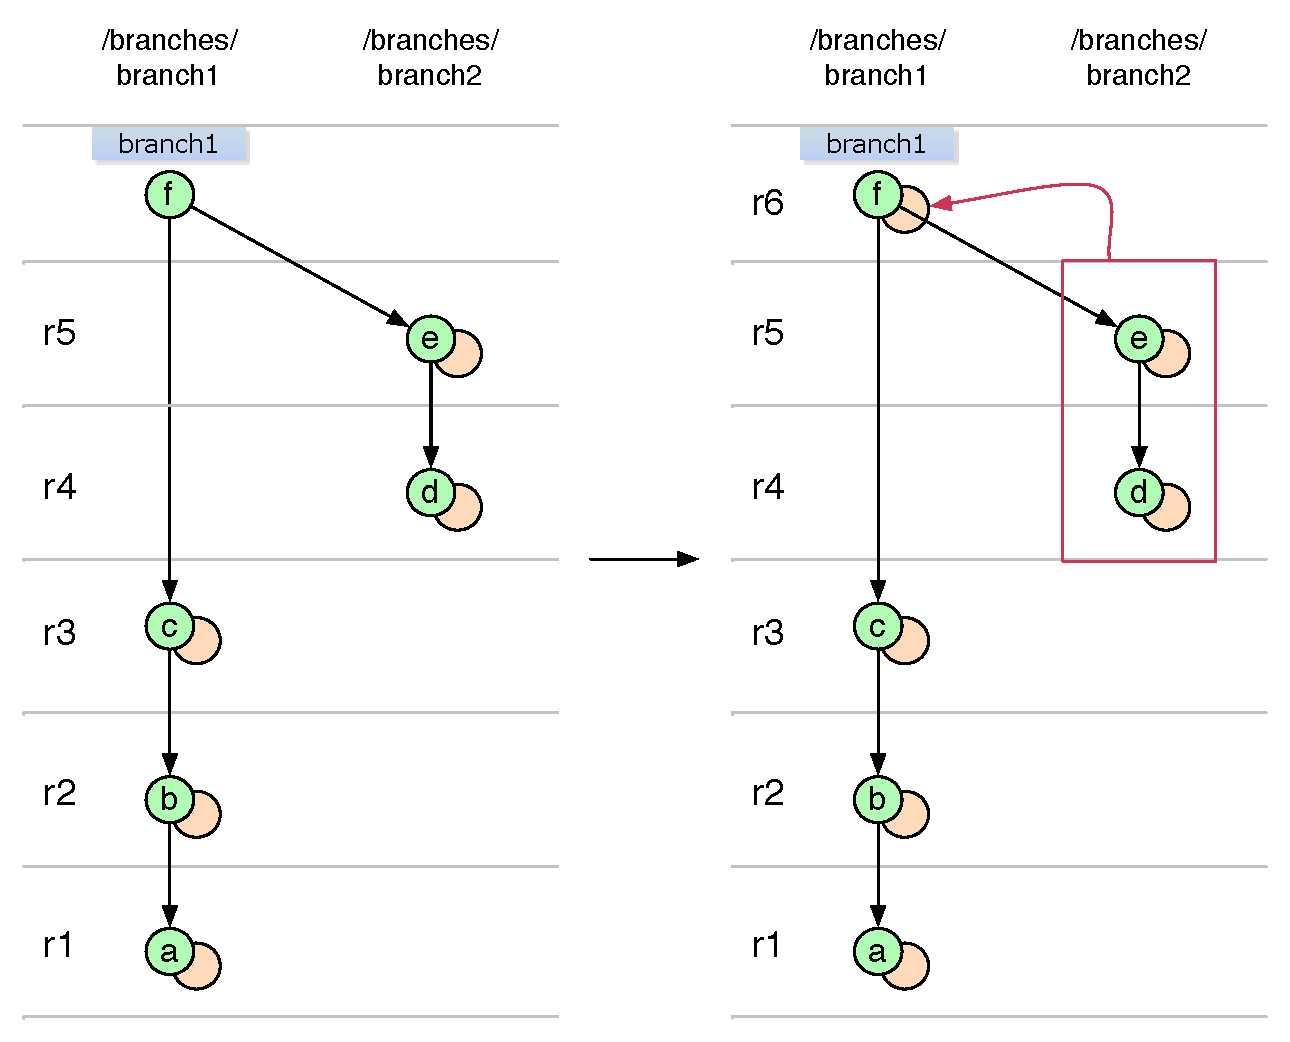
\includegraphics[width=\textwidth]{img/diagrams/simple_merge_branch_no_parent_git_to_svn.pdf}%
\captionof{figure}{Git merge commit being translated to the change of svn:mergeinfo property.}
\label{simple_merge_branch_no_parent_git_to_svn}%
\end{center}

It is natural to reverse this idea for Subversion to Git merge history translation. If revision r3 modified svn:mergeinfo property of branch branch1 that merge history of branch1 includes whole history of branch2, then merge commit should be created for that case. Diagrams \ref{simple_merge_svn_to_git} and \ref{simple_merge_branch_no_parent_svn_to_git} illustrate this approach.

\begin{center}
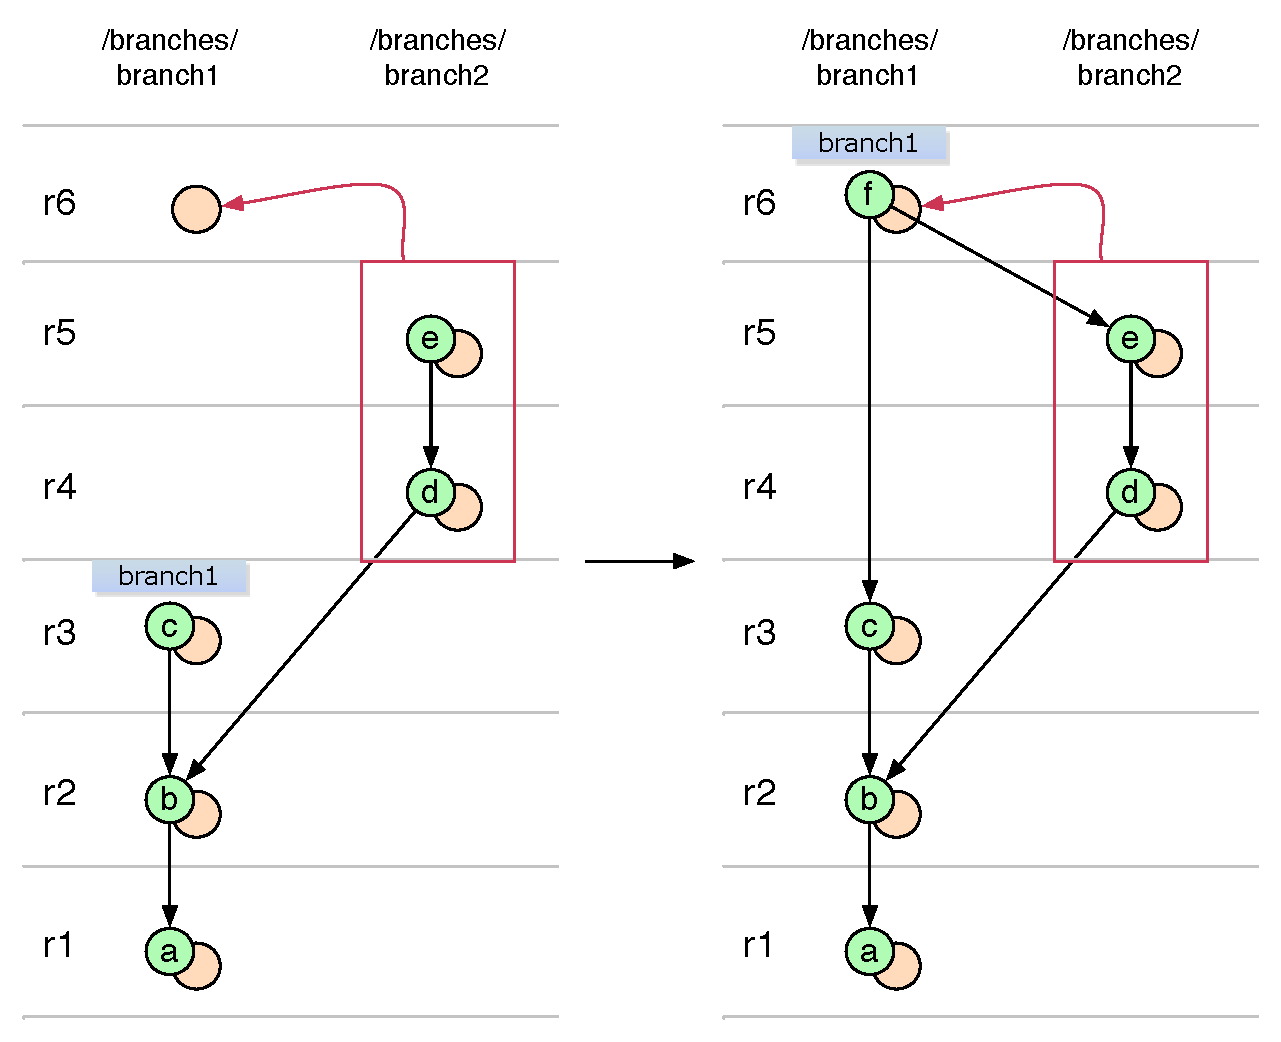
\includegraphics[width=\textwidth]{img/diagrams/simple_merge_svn_to_git.pdf}%
\captionof{figure}{svn:mergeinfo property change being translated into merge commit creation.}
\label{simple_merge_svn_to_git}%
\end{center}

\begin{center}
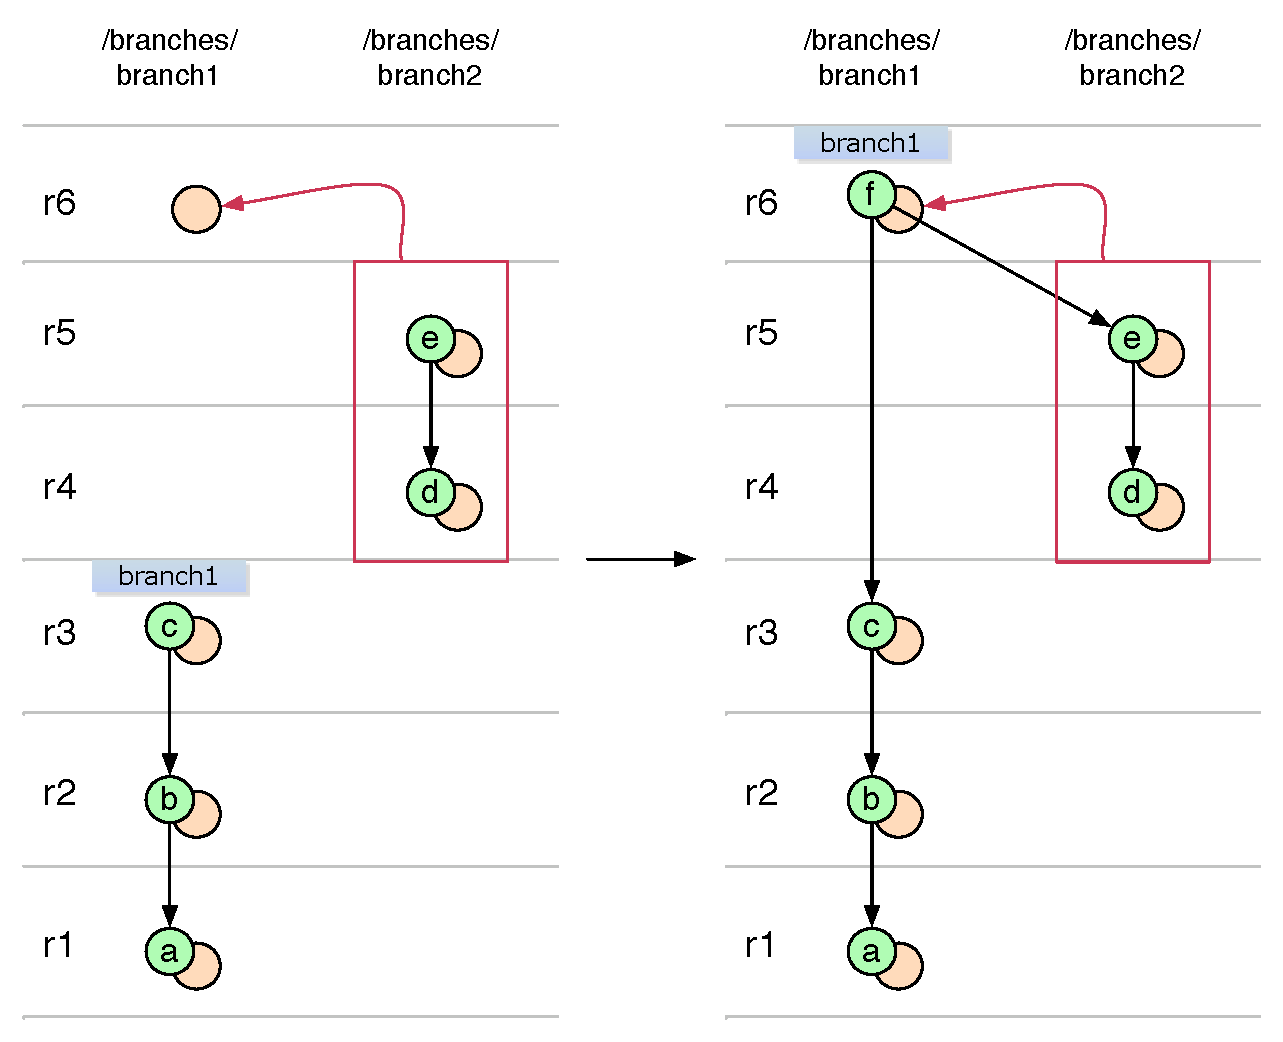
\includegraphics[width=\textwidth]{img/diagrams/simple_merge_branch_no_parent_svn_to_git.pdf}%
\captionof{figure}{svn:mergeinfo property change being translated into merge commit creation.}
\label{simple_merge_branch_no_parent_svn_to_git}%
\end{center}

\subsubsection{Cherry Pick}

Subversion tracks cherry-pick merges as well as merges of the whole branch history. Git doesn't support this kind of merges. Hence cherry-pick merge performed by Subversion user is translated as a new ordinary commit with corresponding changes. This case depicted at diagram \ref{no_merge_commit_on_cherry_pick_svn_to_git}.

\begin{center}
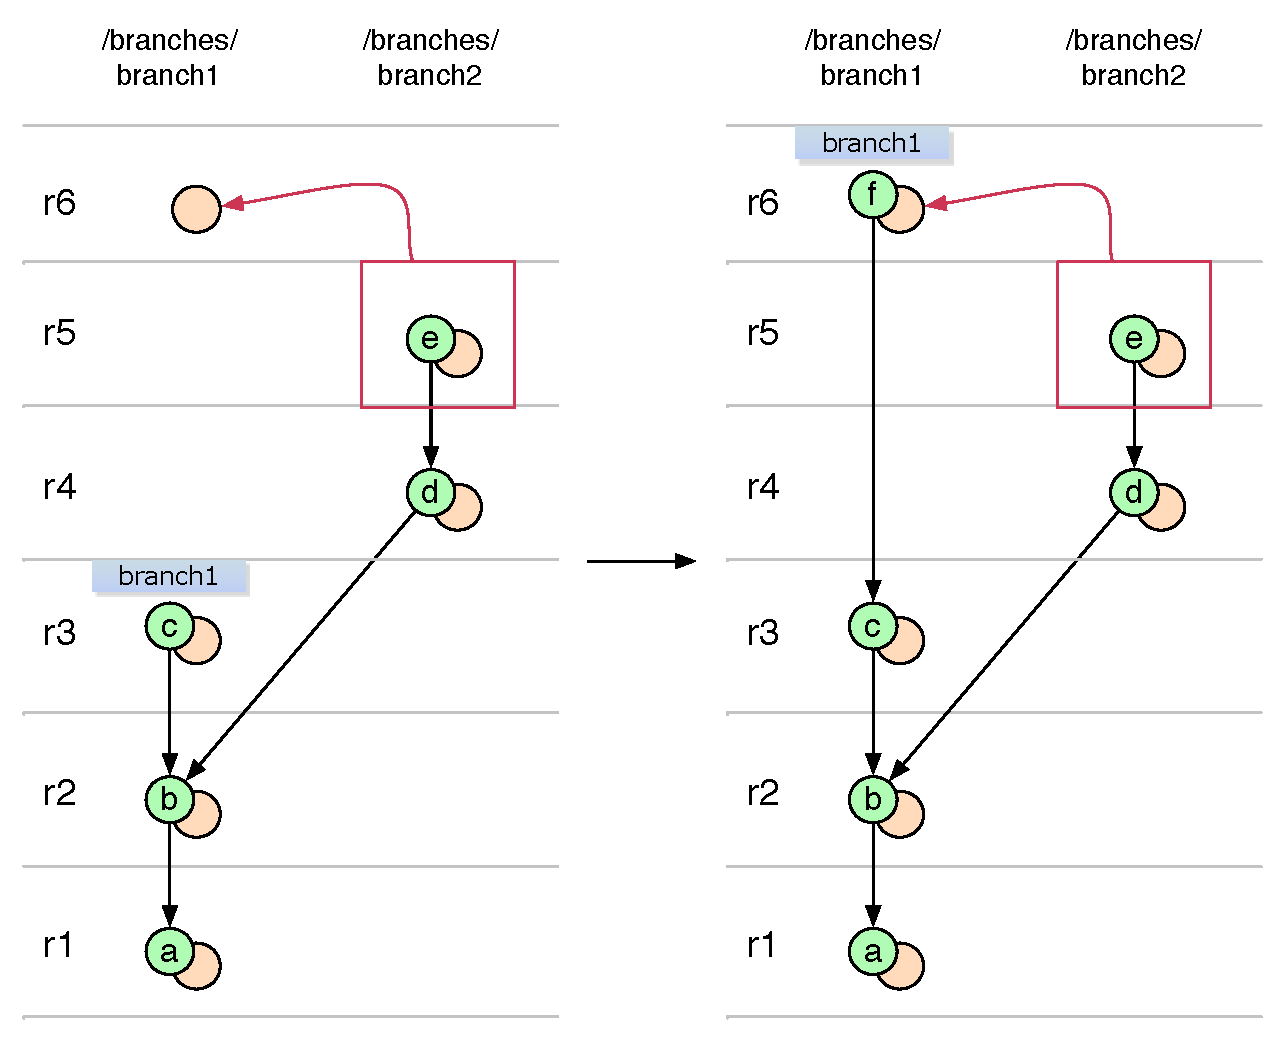
\includegraphics[width=\textwidth]{img/diagrams/no_merge_commit_on_cherry_pick_svn_to_git.pdf}%
\captionof{figure}{Cherry-pick merge being translated to ordinary commit.}
\label{no_merge_commit_on_cherry_pick_svn_to_git}%
\end{center}

Though a sequence of cherry-pick merges may lead the history of certain branch to the state when it includes the history of another branch as merge history. This scenario is depicted at diagrams \ref{merge_commit_on_double_cherry_pick_svn_to_git} and \ref{merge_commit_on_double_cherry_pick_branch_no_parent_svn_to_git}.

\begin{center}
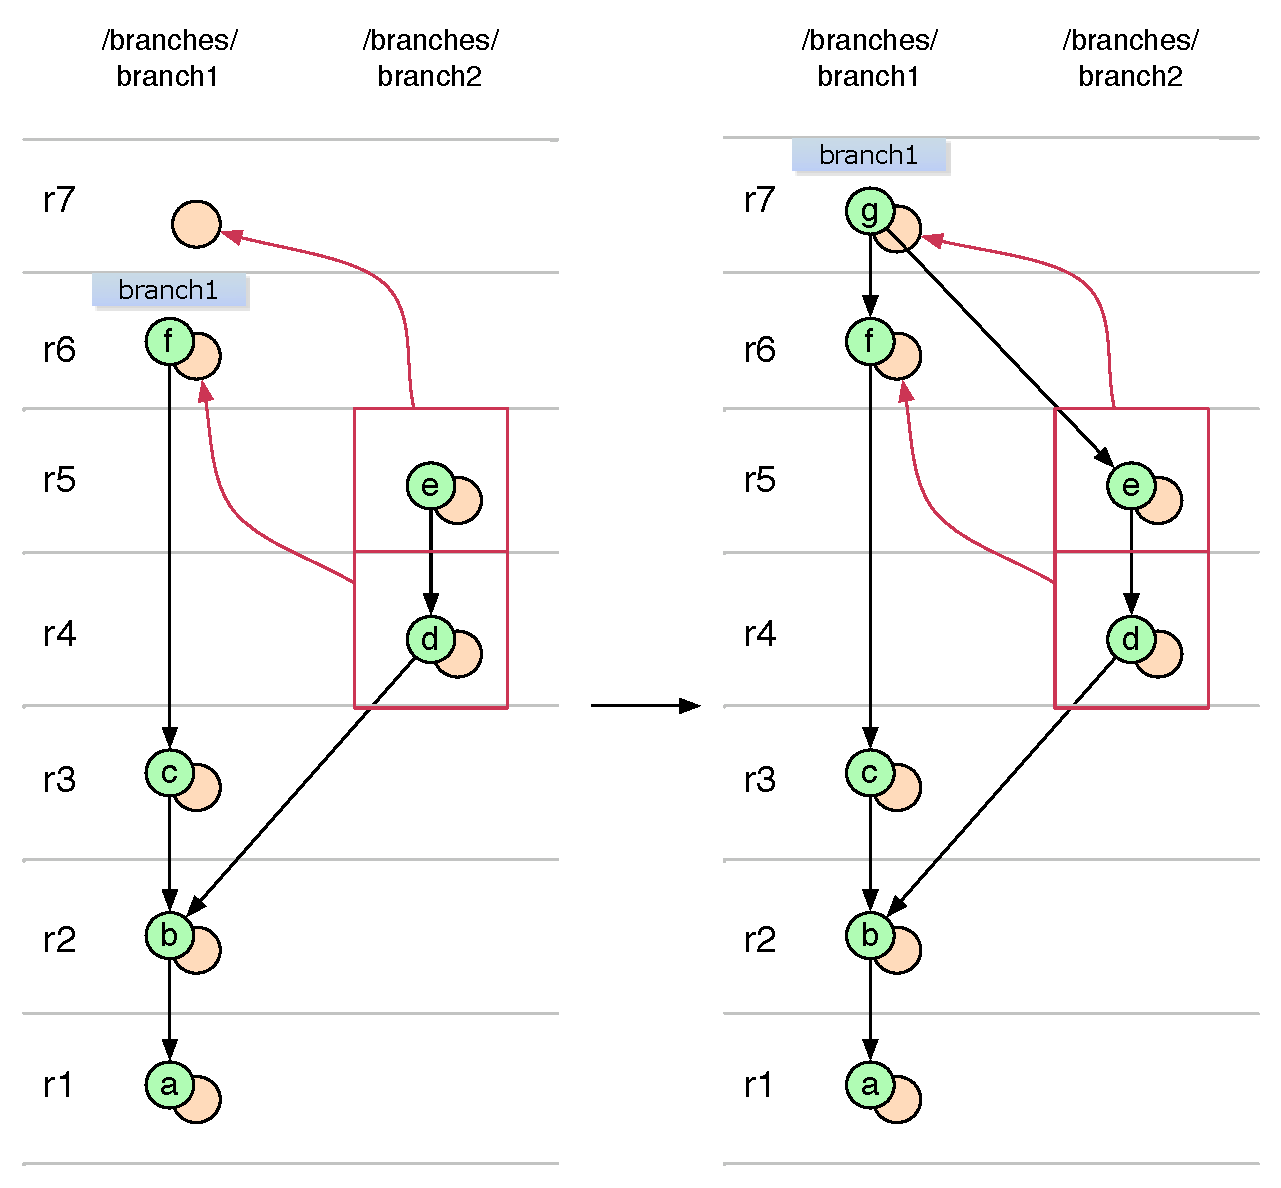
\includegraphics[width=\textwidth]{img/diagrams/merge_commit_on_double_cherry_pick_svn_to_git.pdf}%
\captionof{figure}{Merge of unnamed Git branch being translated to a sequence of Subversion revisions.}
\label{merge_commit_on_double_cherry_pick_svn_to_git}%
\end{center}

\begin{center}
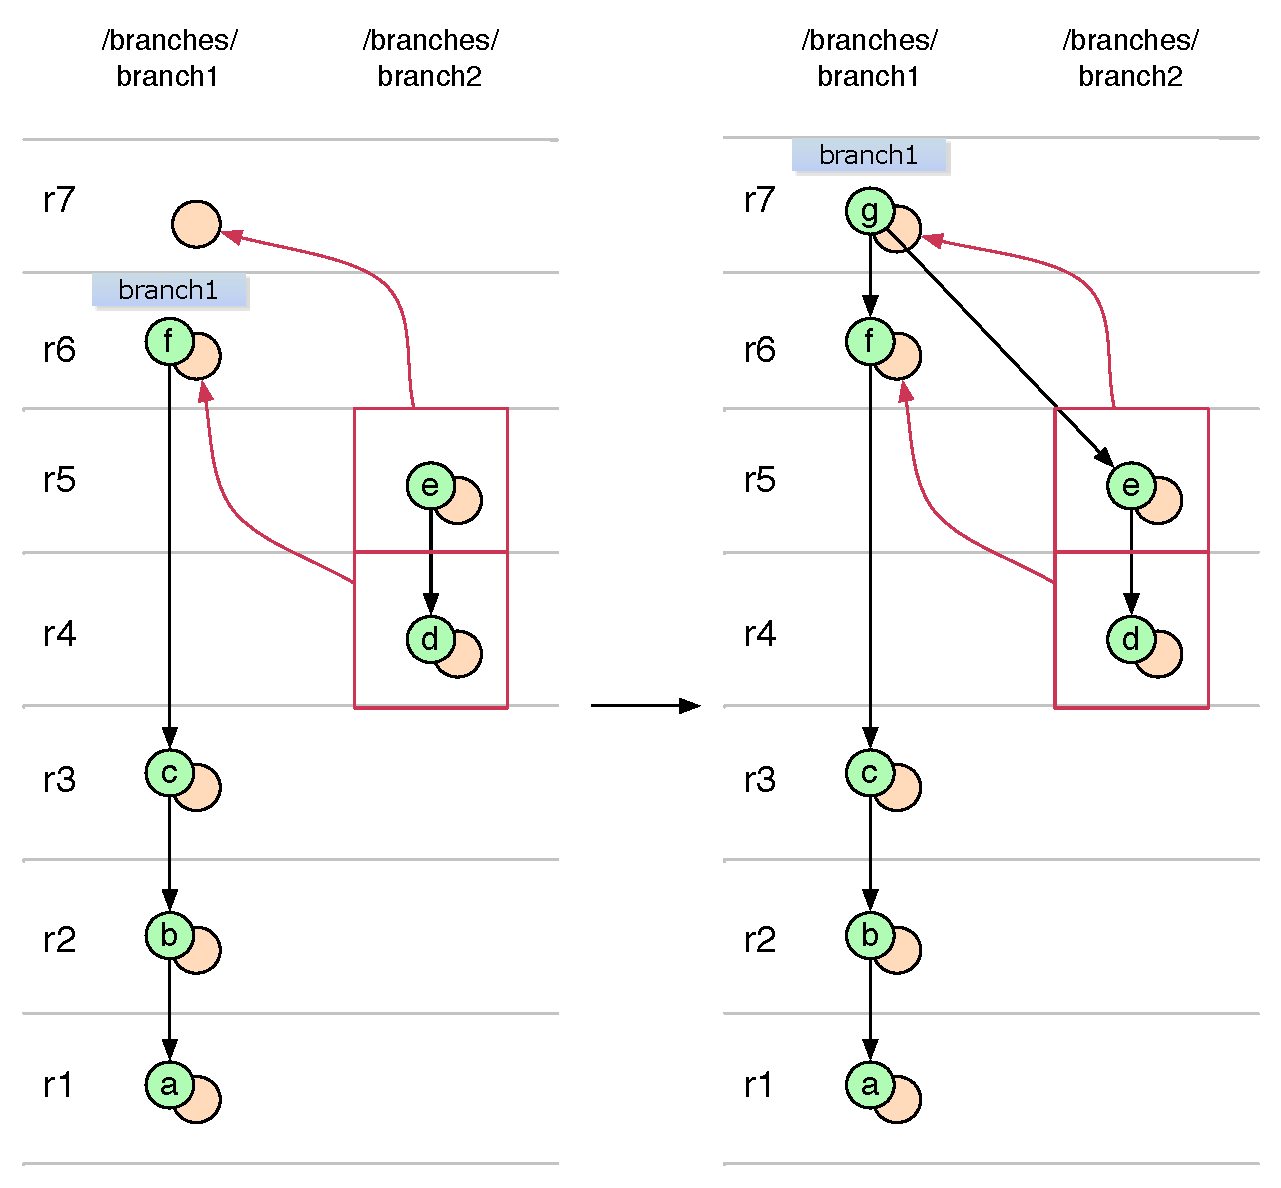
\includegraphics[width=\textwidth]{img/diagrams/merge_commit_on_double_cherry_pick_branch_no_parent_svn_to_git.pdf}%
\captionof{figure}{Merge of unnamed Git branch being translated to a sequence of Subversion revisions.}
\label{merge_commit_on_double_cherry_pick_branch_no_parent_svn_to_git}%
\end{center}

\subsubsection{Shelve Branches}

\begin{center}
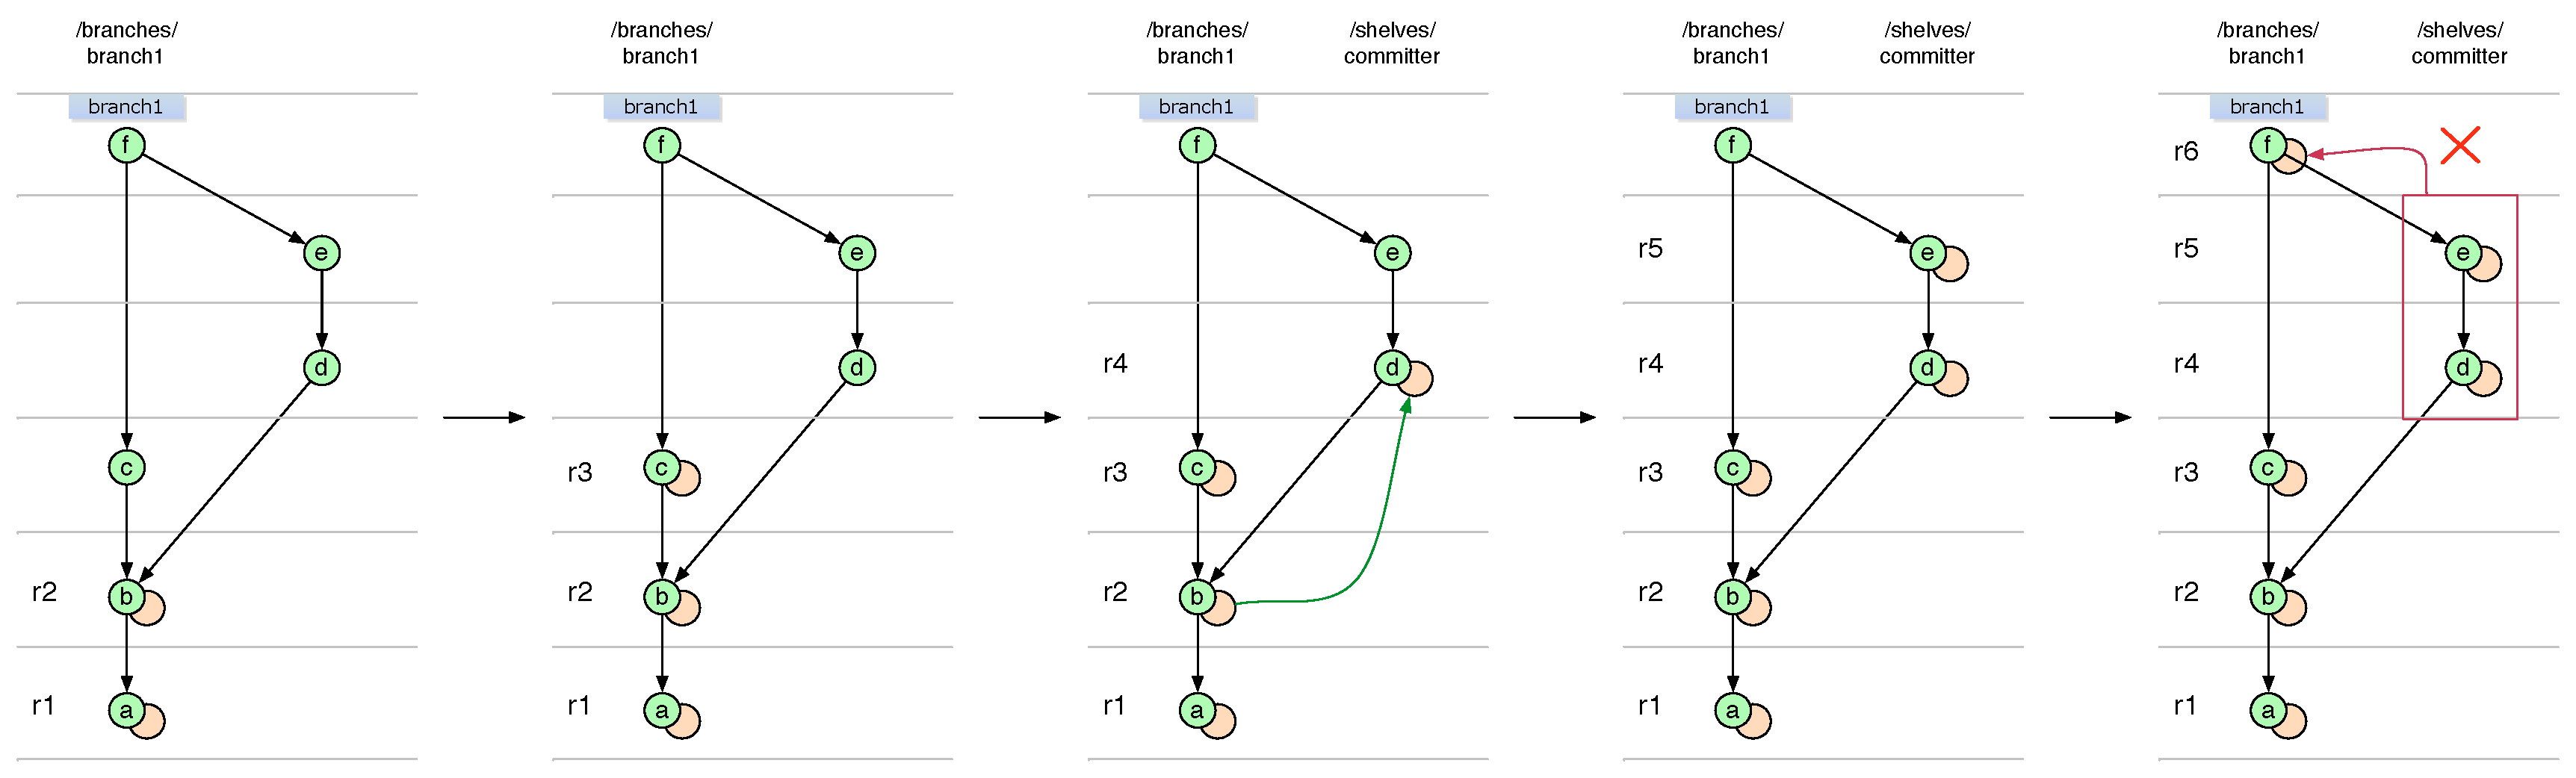
\includegraphics[width=\textwidth]{img/diagrams/boat_merge_git_to_svn.pdf}%
\captionof{figure}{Merge of unnamed Git branch being translated to a sequence of Subversion revisions.}
\label{boat_merge_git_to_svn}%
\end{center}

\begin{center}
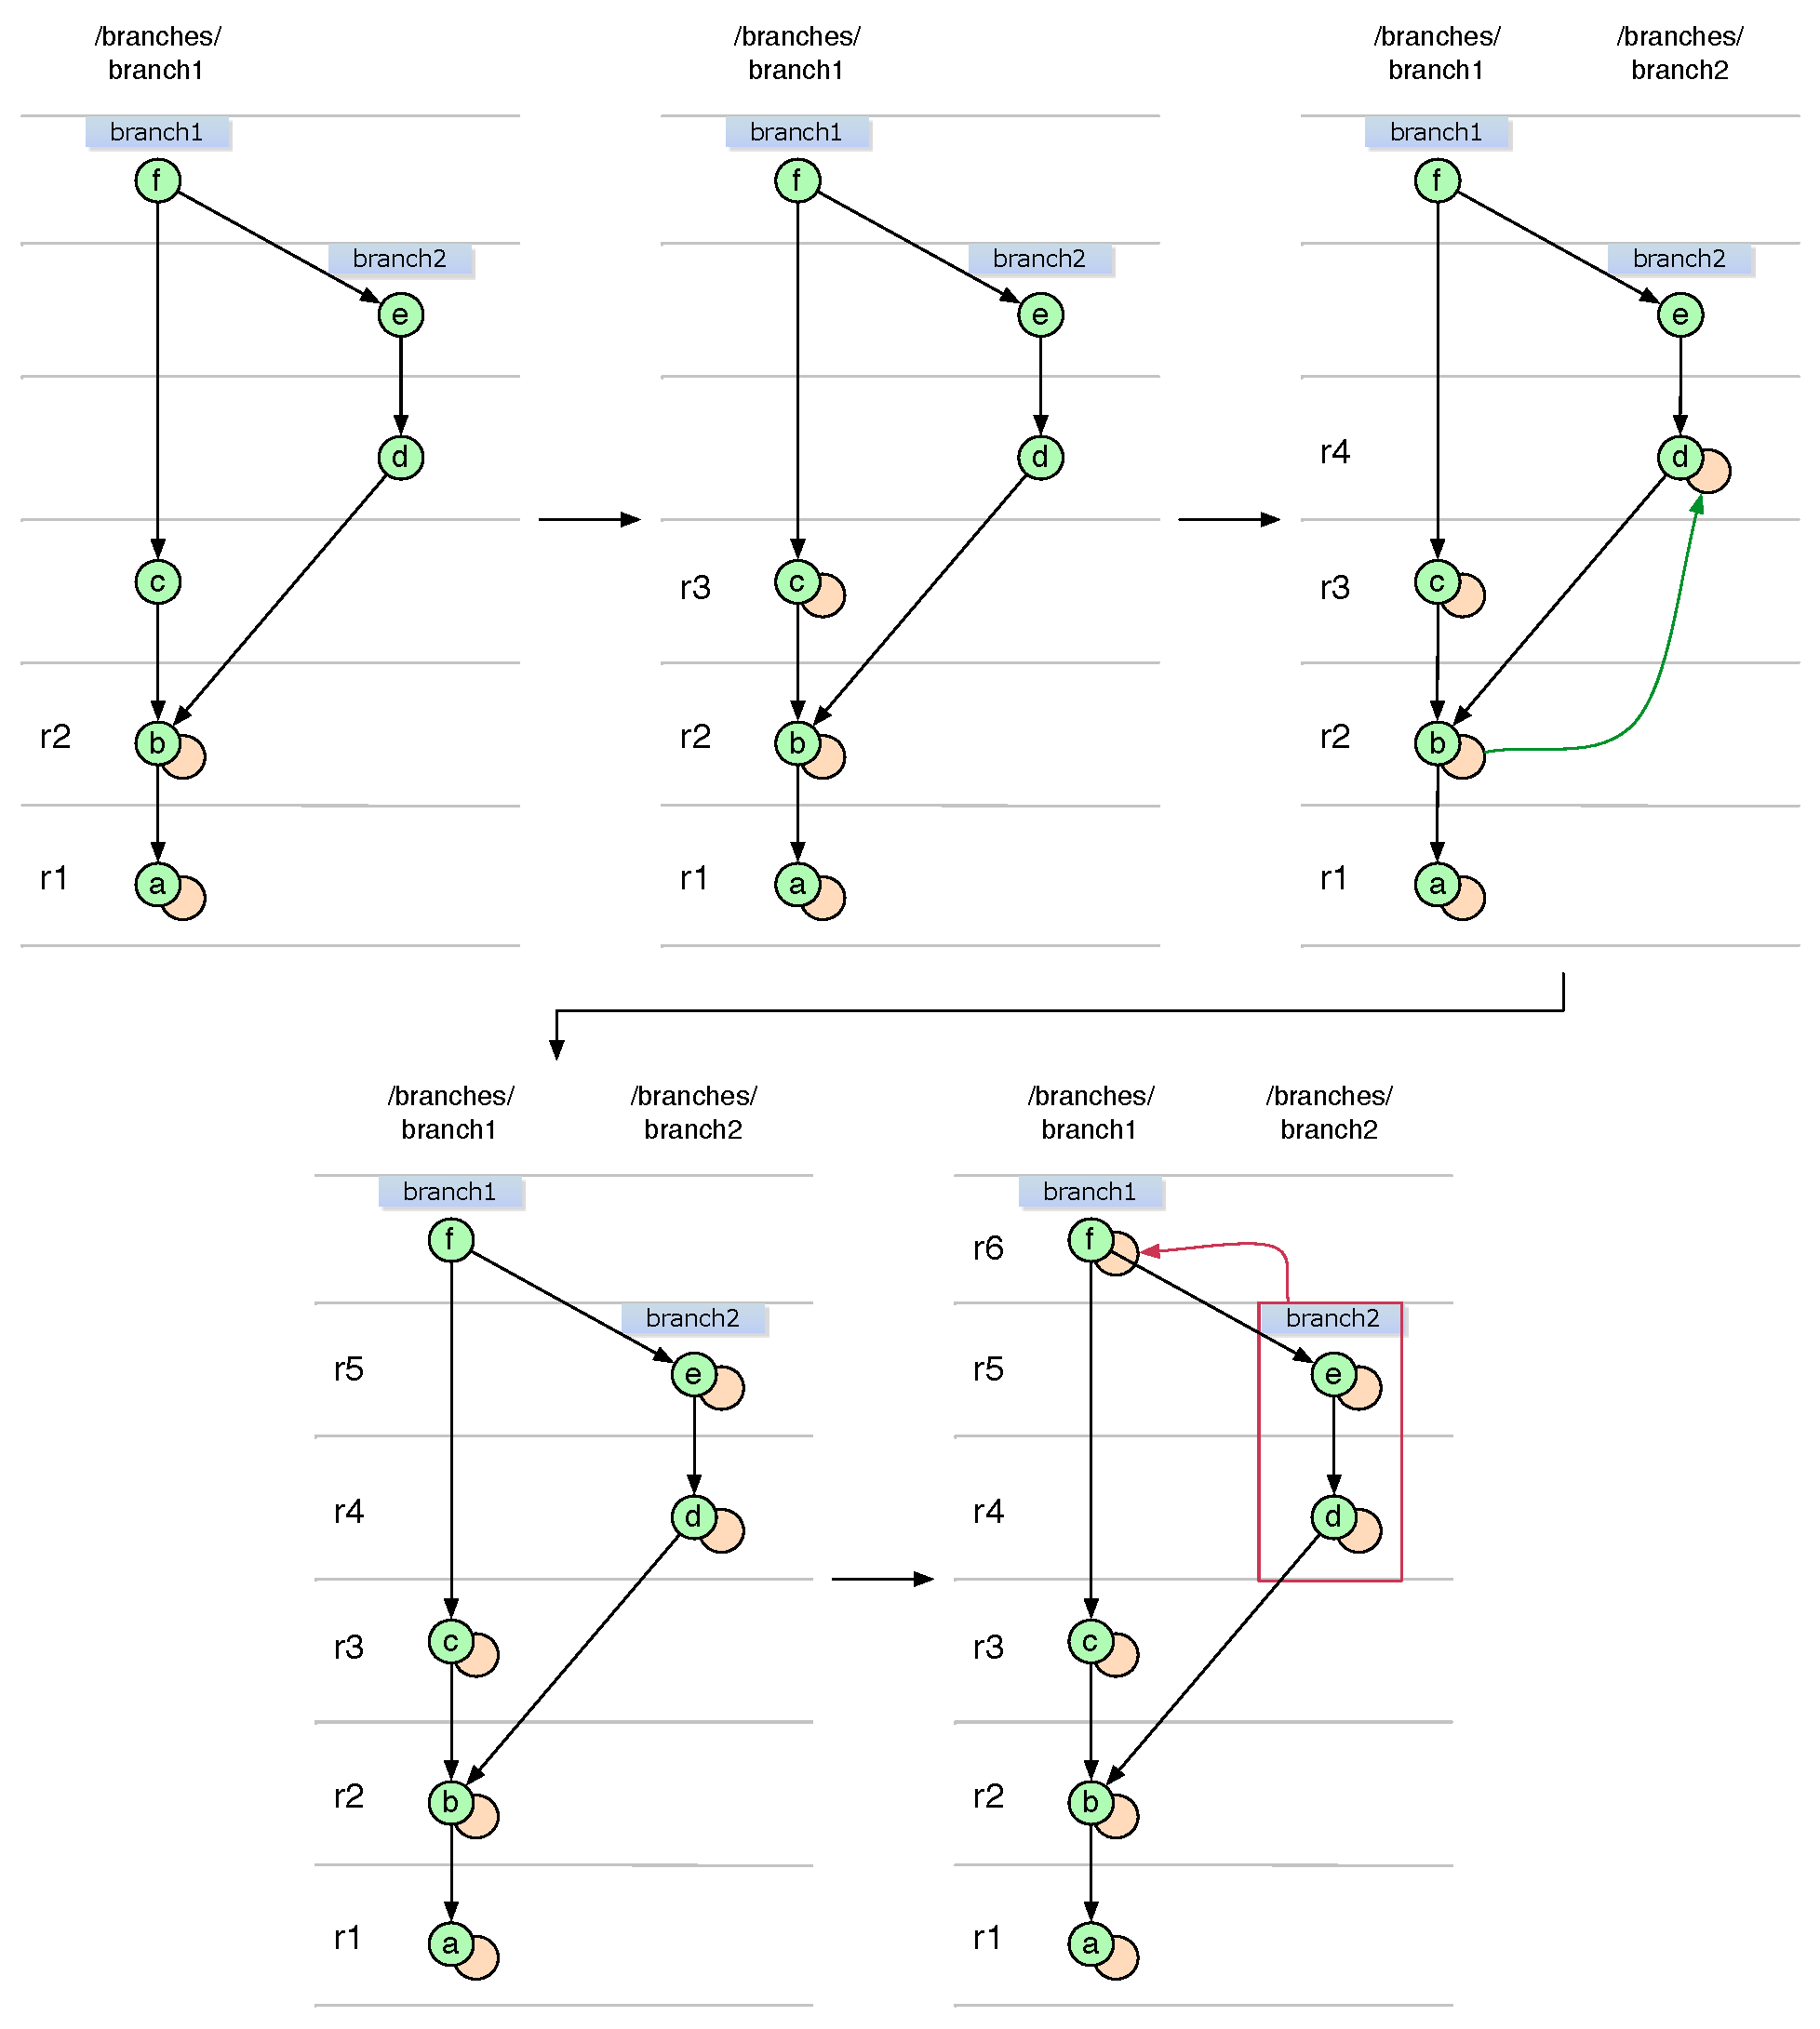
\includegraphics[width=\textwidth]{img/diagrams/boat_merge_named_shelve_git_to_svn.pdf}%
\captionof{figure}{Merge of Git branch which is available from another branch being translated to a sequence of Subversion revisions.}
\label{boat_merge_named_shelve_git_to_svn}%
\end{center}

\begin{center}
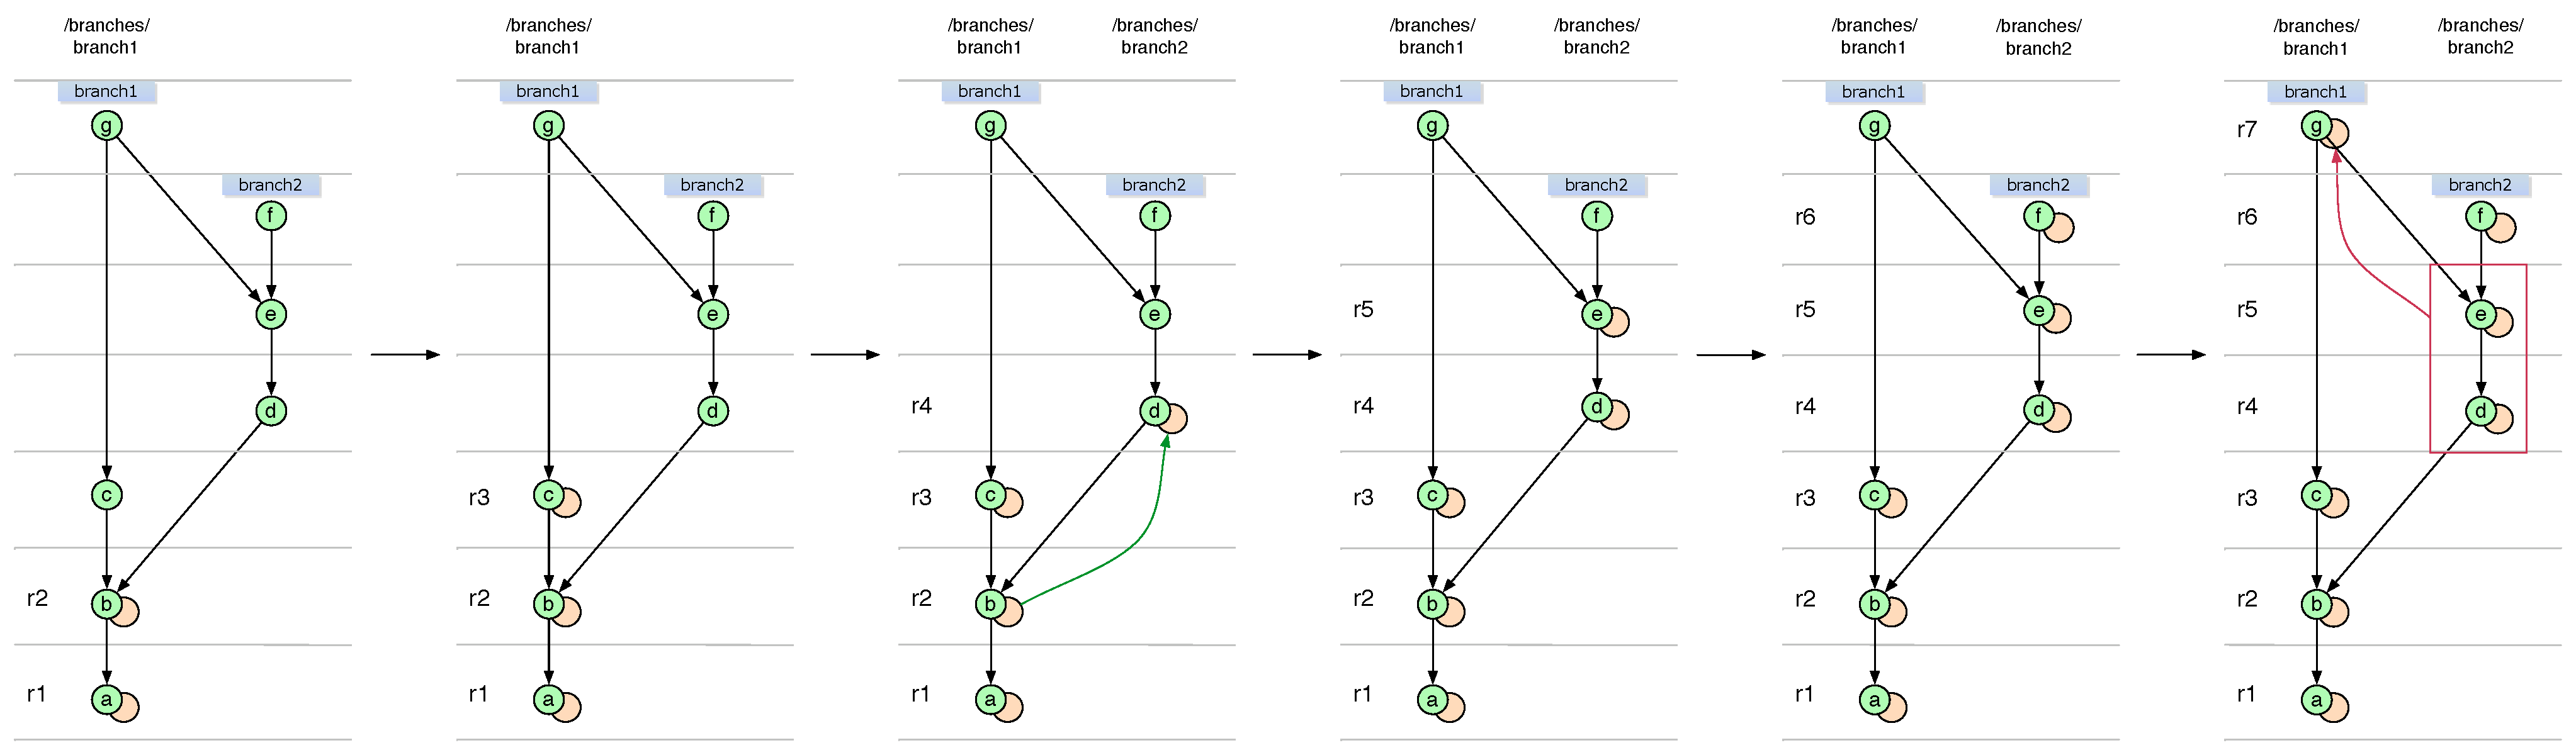
\includegraphics[width=\textwidth]{img/diagrams/boat_merge_shelve_is_normal_branch_git_to_svn.pdf}%
\captionof{figure}{Merge of Git branch which is available from another branch being translated to a sequence of Subversion revisions.}
\label{boat_merge_shelve_is_normal_branch_git_to_svn}%
\end{center}

\subsubsection{Nested Merge}

\begin{center}
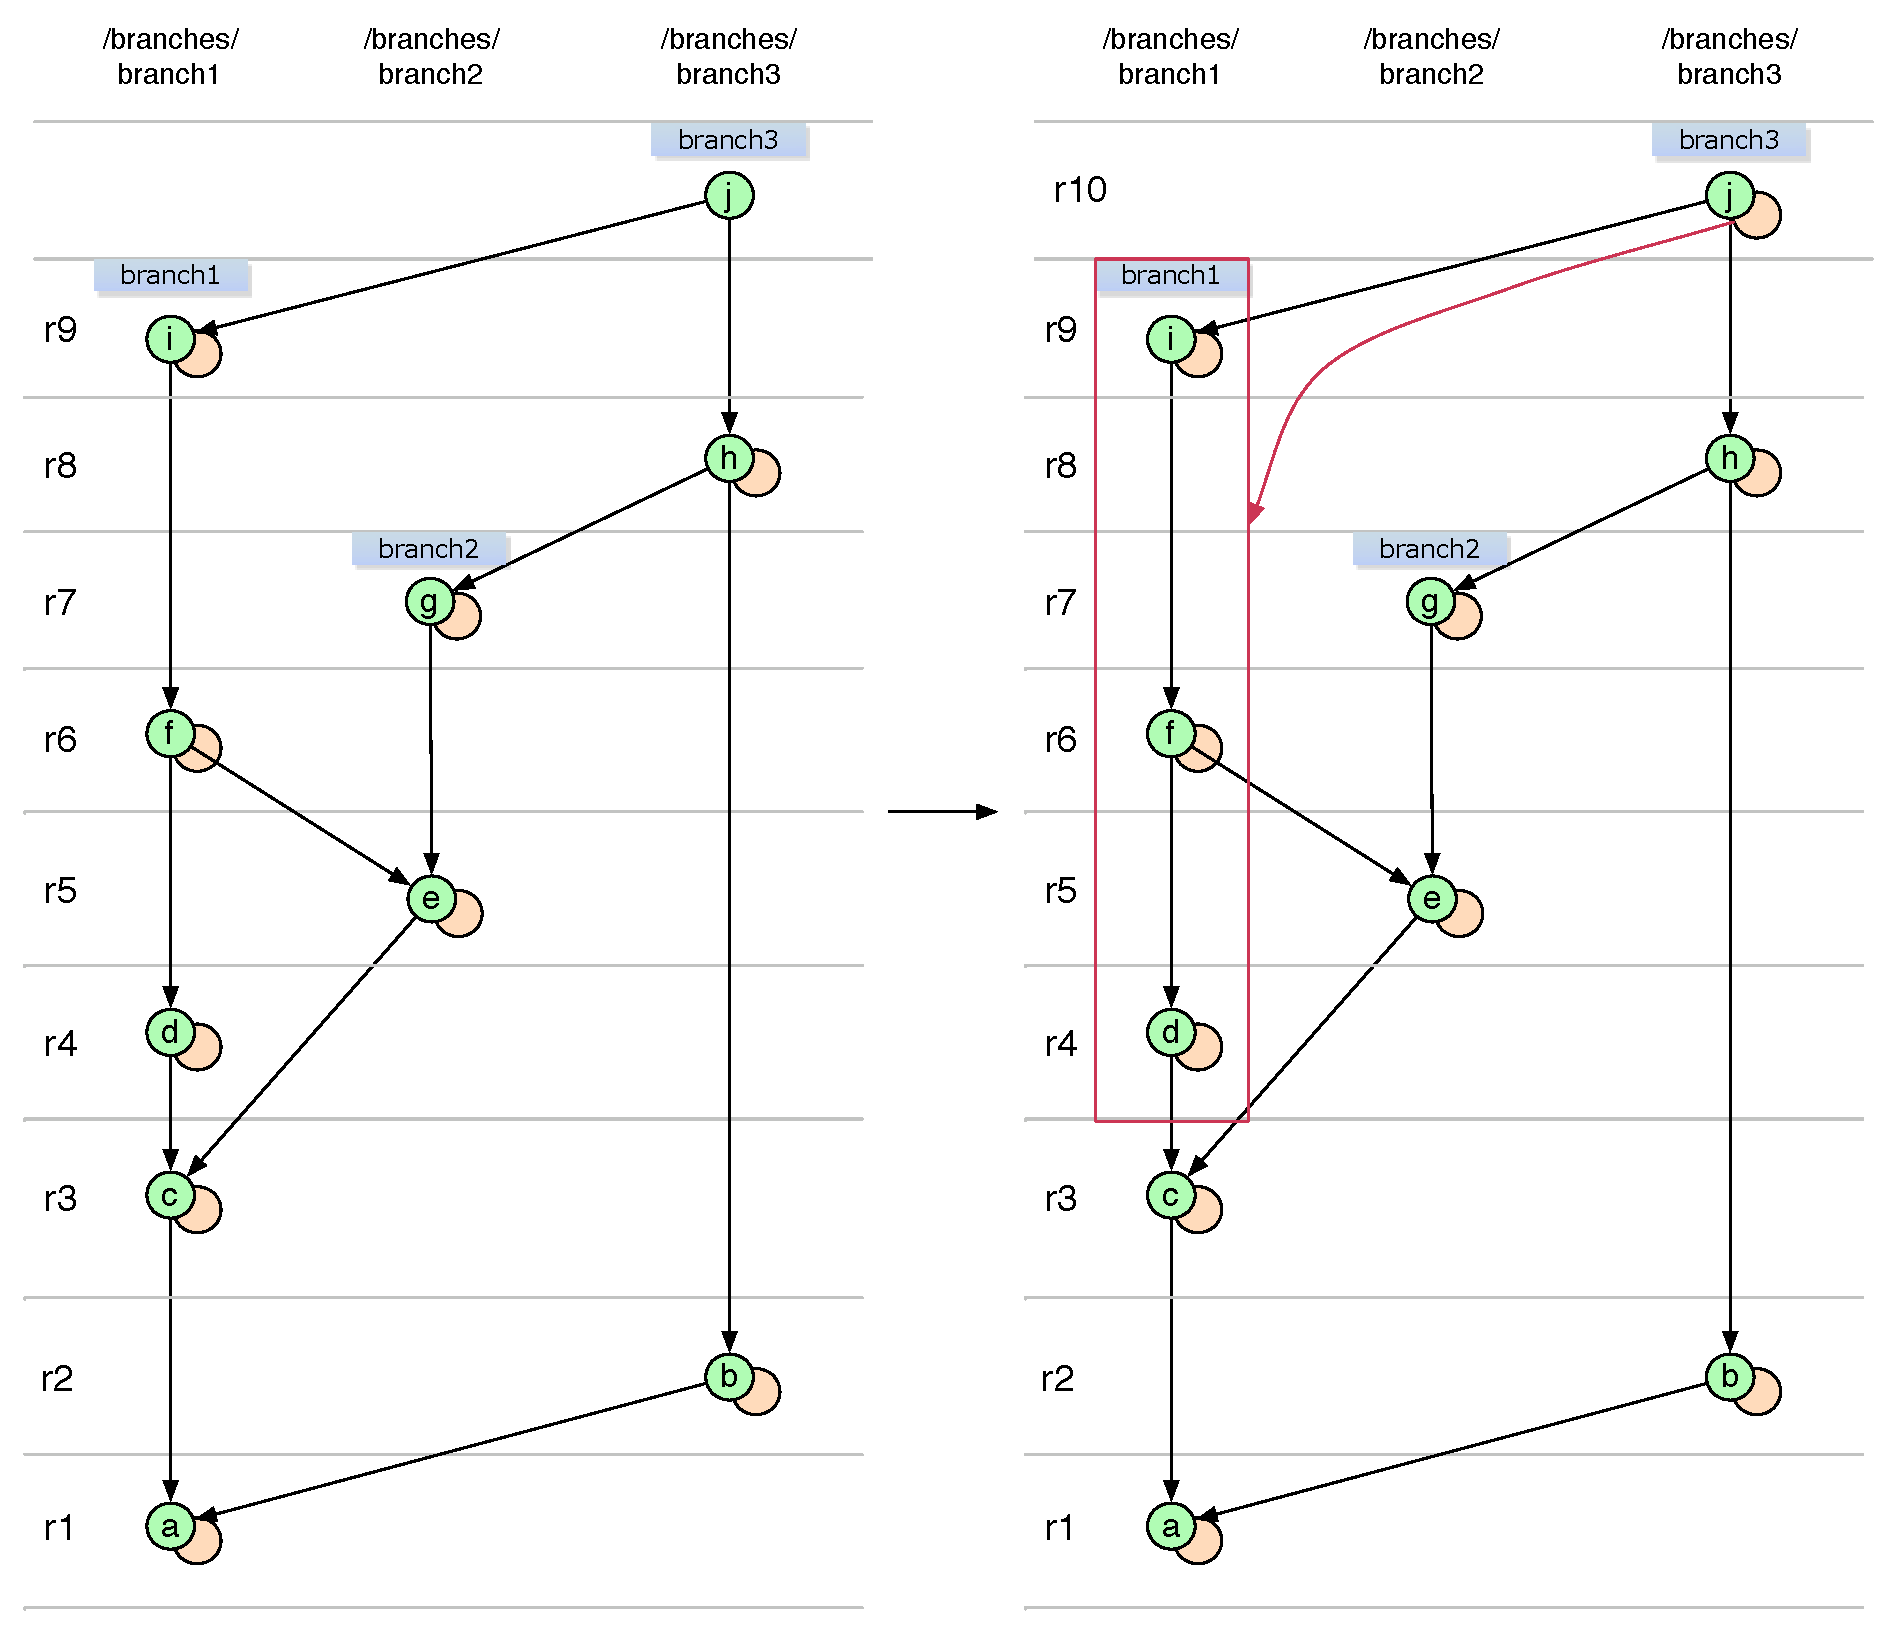
\includegraphics[width=\textwidth]{img/diagrams/merge_sequence_git_to_svn.pdf}%
\captionof{figure}{Merge of Git branch which is available from another branch being translated to a sequence of Subversion revisions.}
\label{merge_sequence_git_to_svn}%
\end{center}

\begin{center}
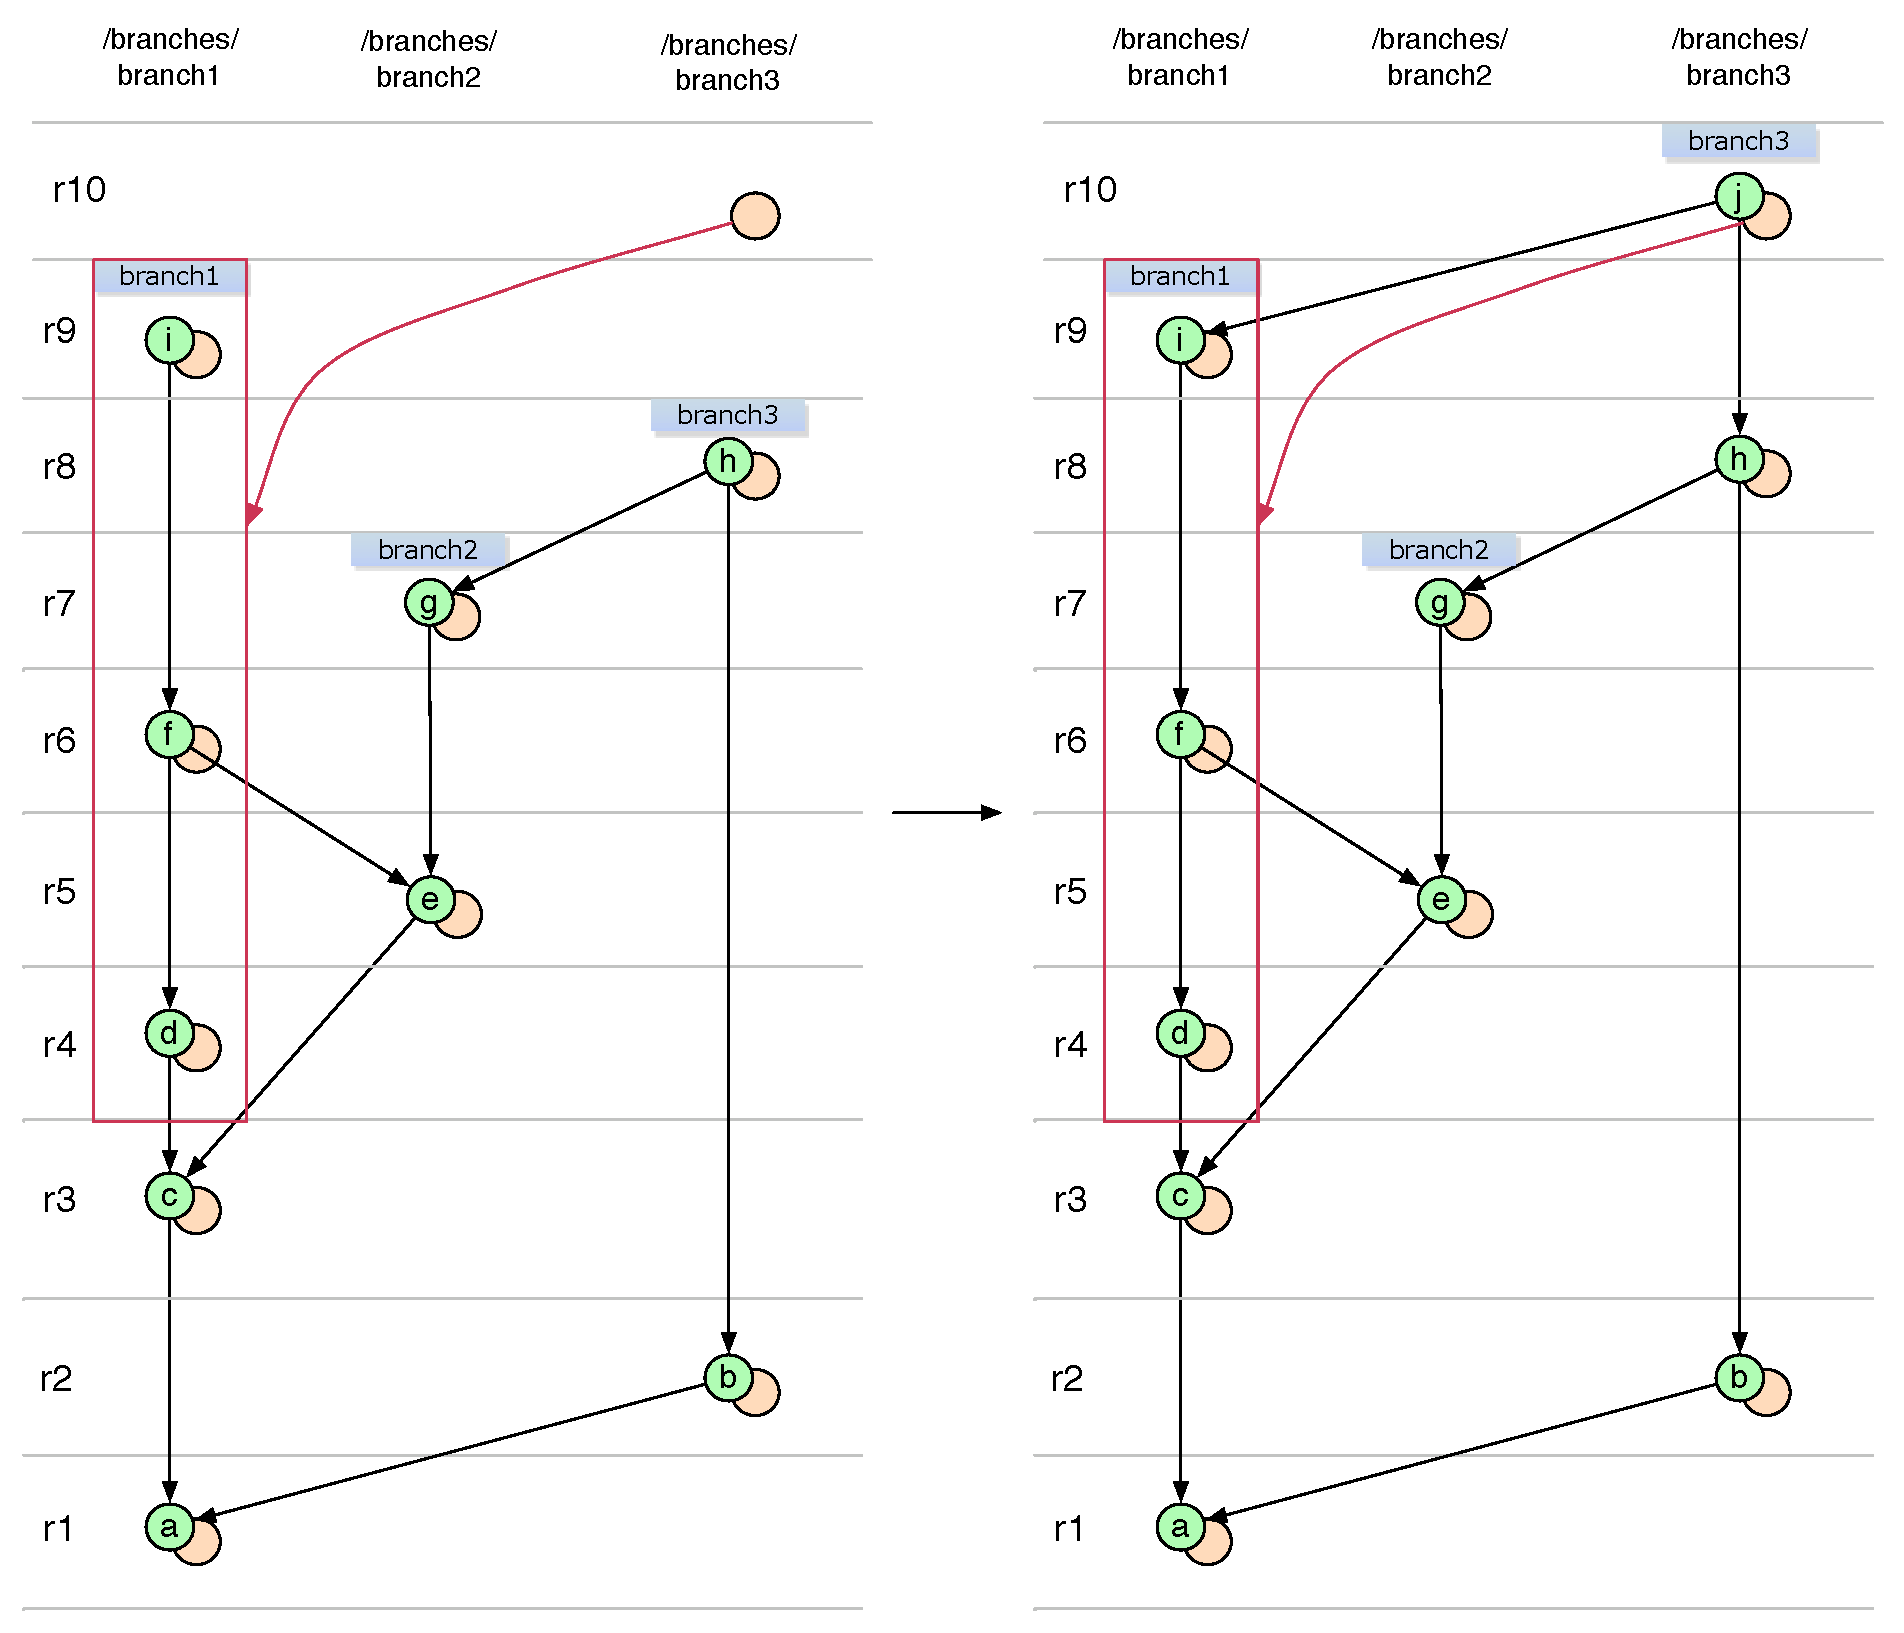
\includegraphics[width=\textwidth]{img/diagrams/merge_sequence_svn_to_git.pdf}%
\captionof{figure}{Merge of Git branch which is available from another branch being translated to a sequence of Subversion revisions.}
\label{merge_sequence_svn_to_git}%
\end{center}

\begin{center}
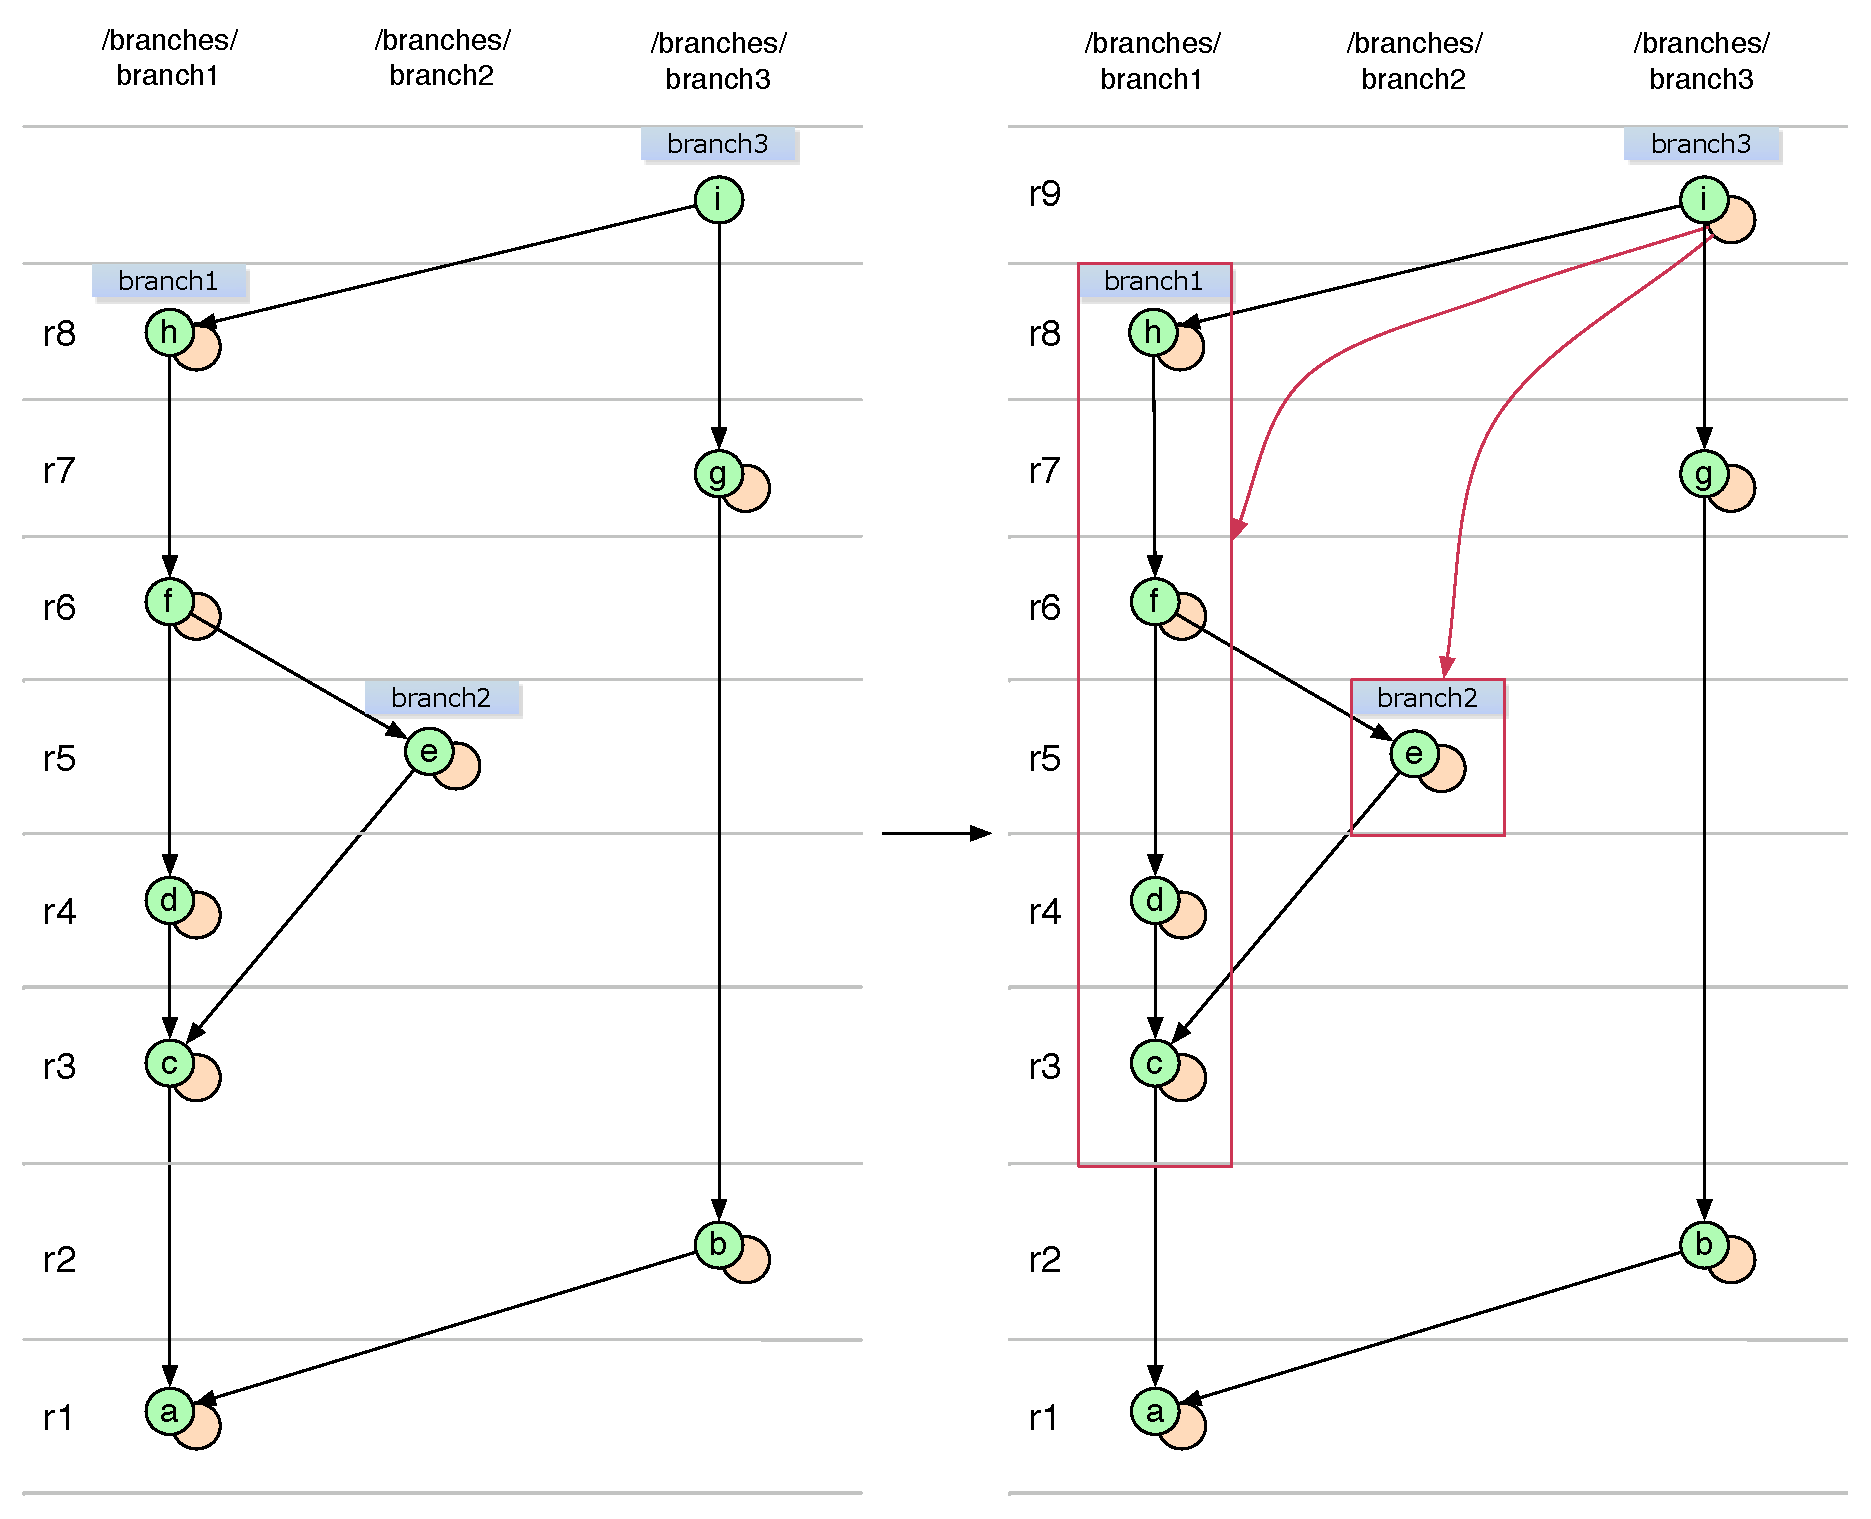
\includegraphics[width=\textwidth]{img/diagrams/nested_merge_full_mergeinfo_git_to_svn.pdf}%
\captionof{figure}{Merge of Git branch which is available from another branch being translated to a sequence of Subversion revisions.}
\label{nested_merge_full_mergeinfo_git_to_svn}%
\end{center}

\begin{center}
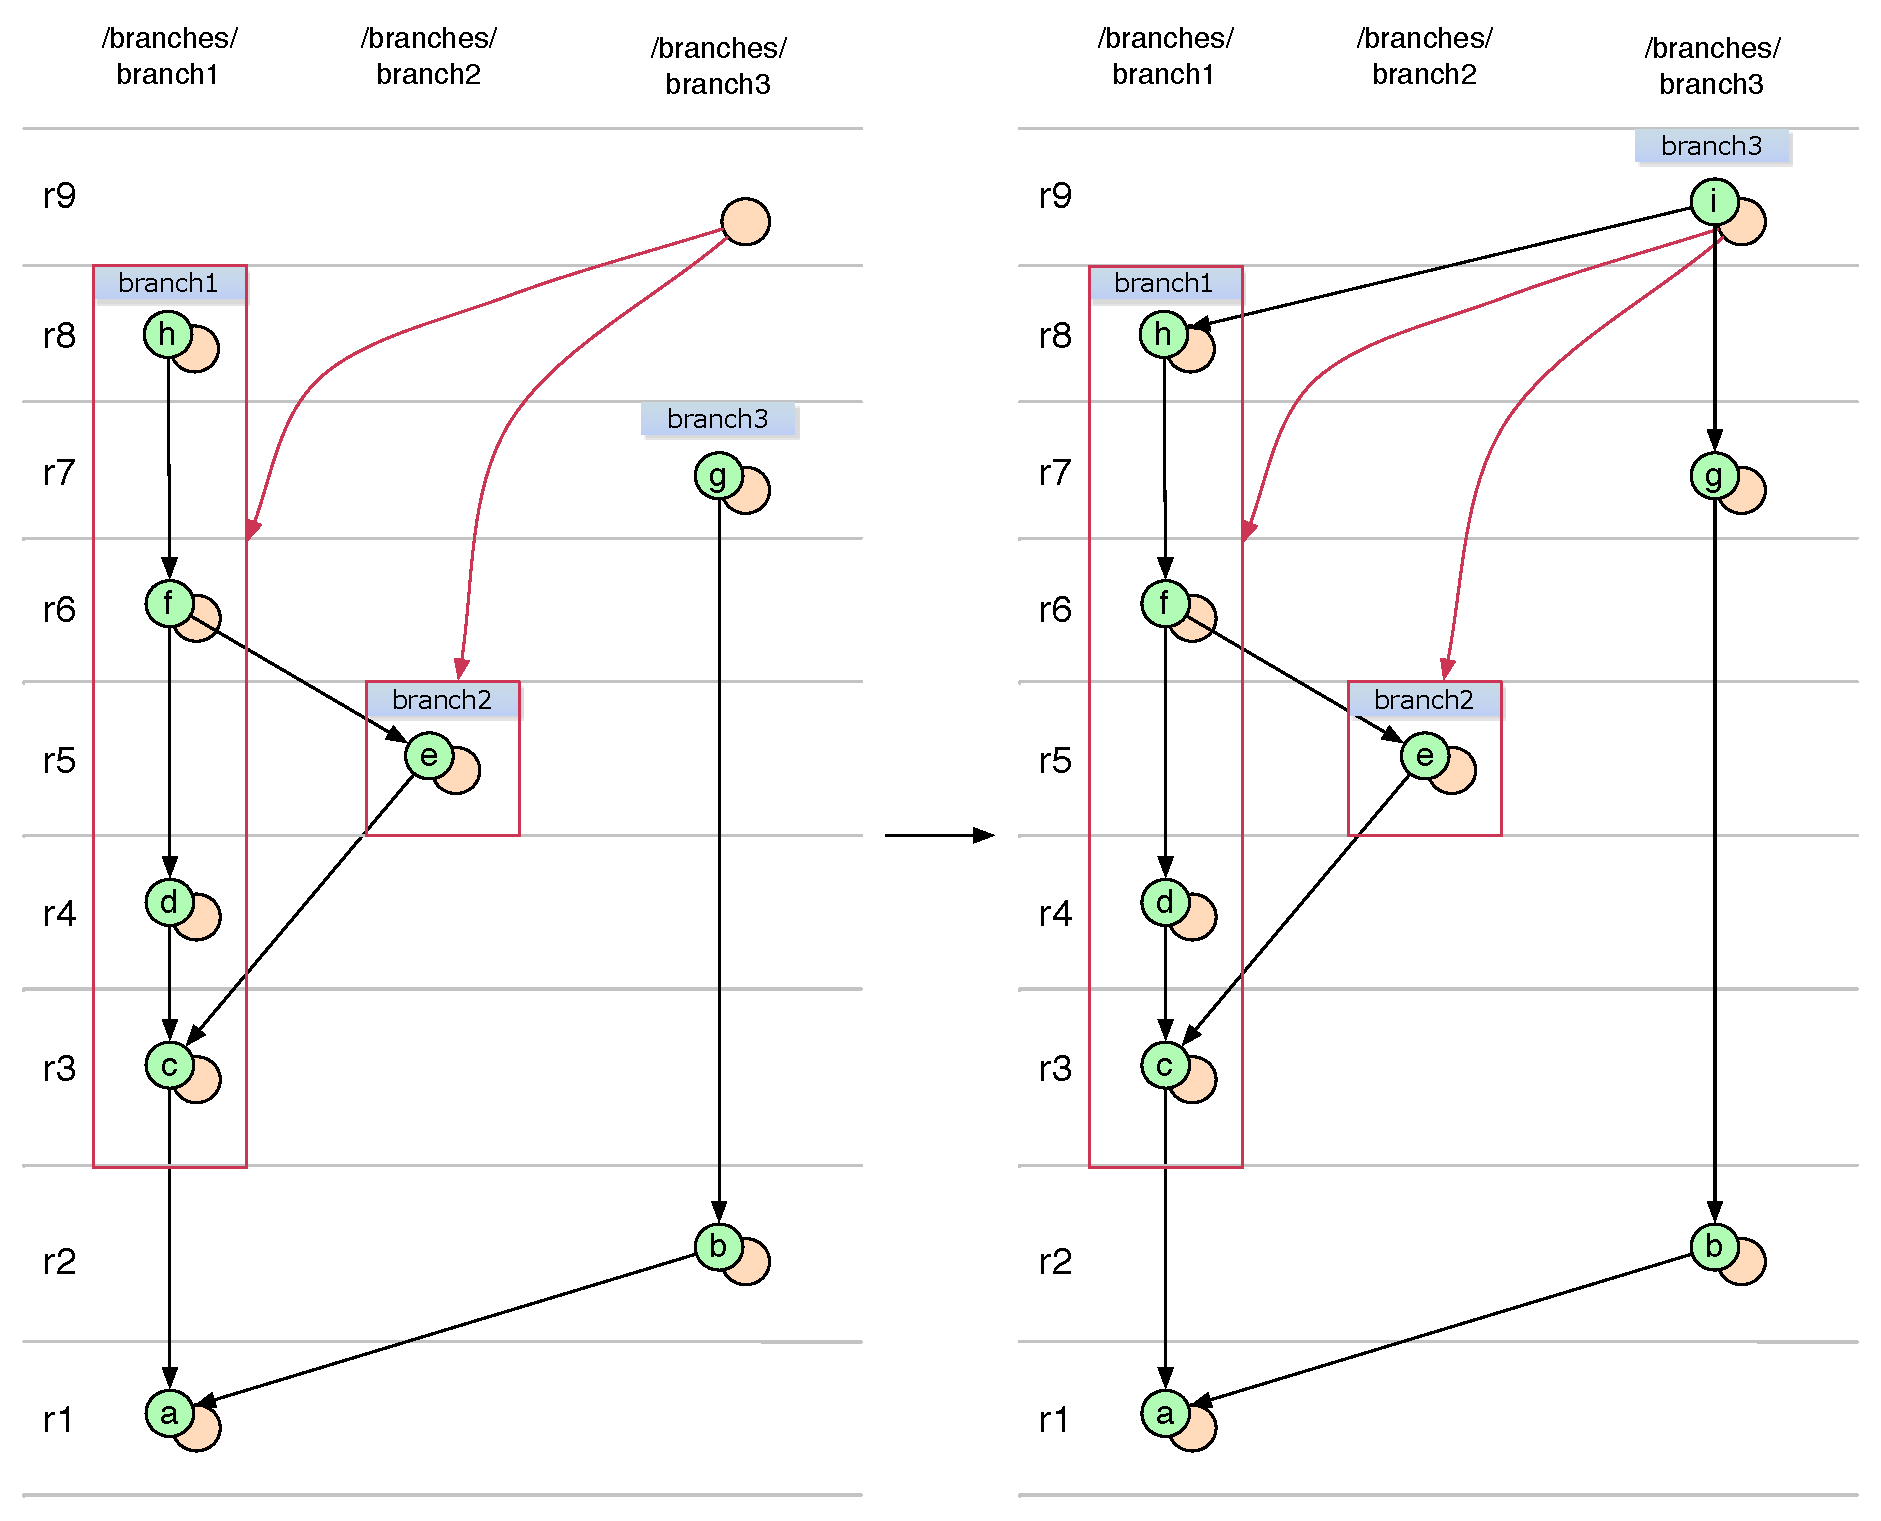
\includegraphics[width=\textwidth]{img/diagrams/nested_merge_full_mergeinfo_svn_to_git.pdf}%
\captionof{figure}{Merge of Git branch which is available from another branch being translated to a sequence of Subversion revisions.}
\label{nested_merge_full_mergeinfo_svn_to_git}%
\end{center}

\begin{center}
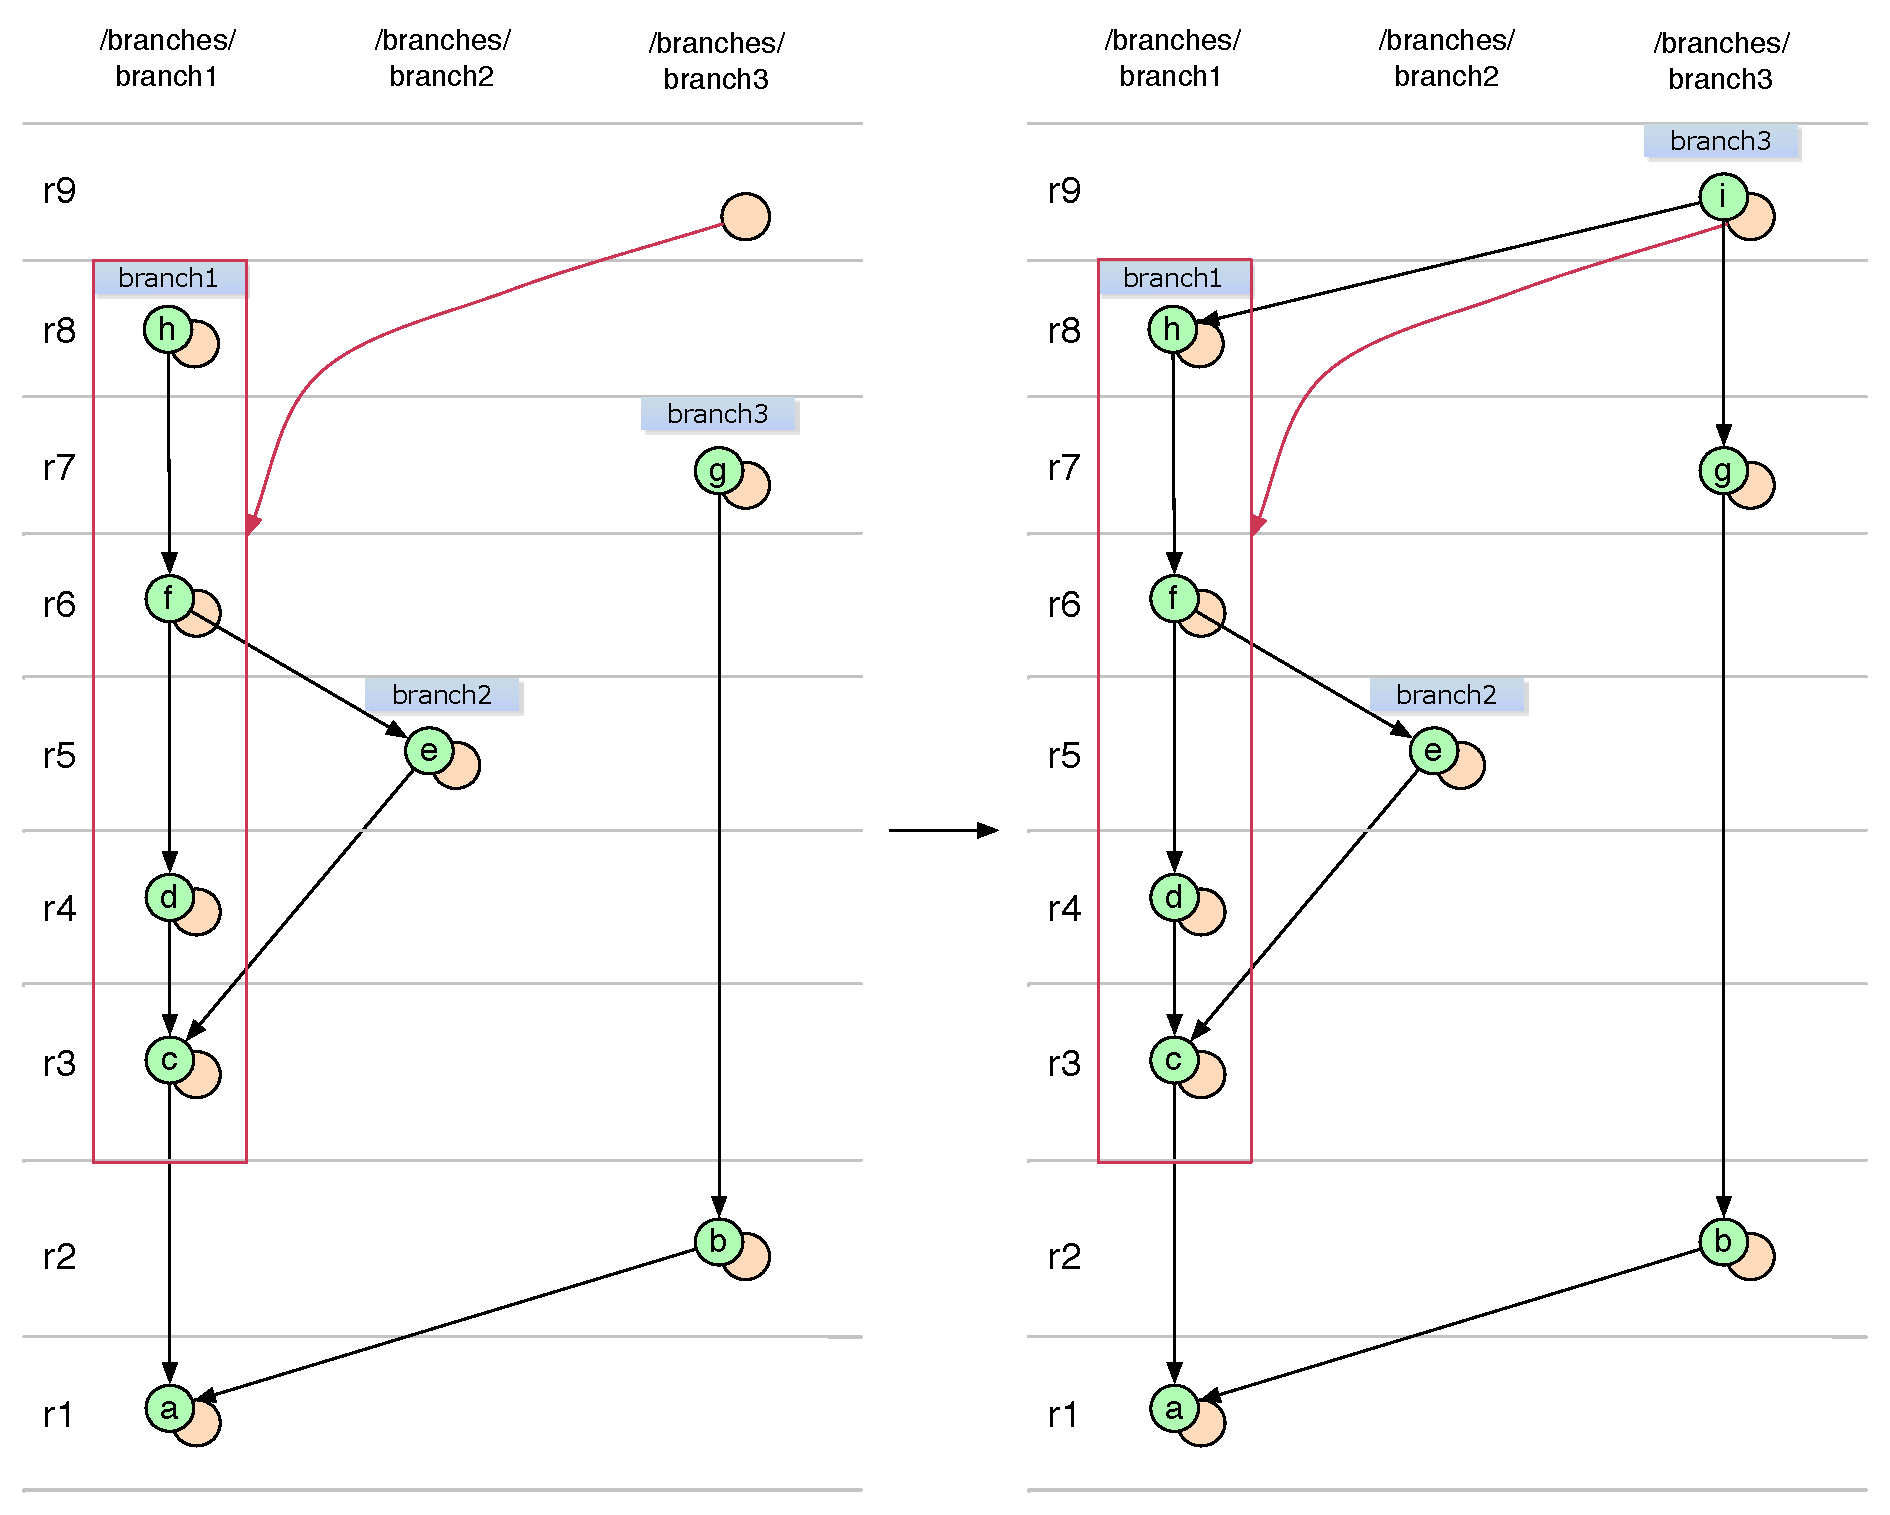
\includegraphics[width=\textwidth]{img/diagrams/nested_merge_partly_mergeinfo_svn_to_git.pdf}%
\captionof{figure}{Merge of Git branch which is available from another branch being translated to a sequence of Subversion revisions.}
\label{nested_merge_partly_mergeinfo_svn_to_git}%
\end{center}

\begin{center}
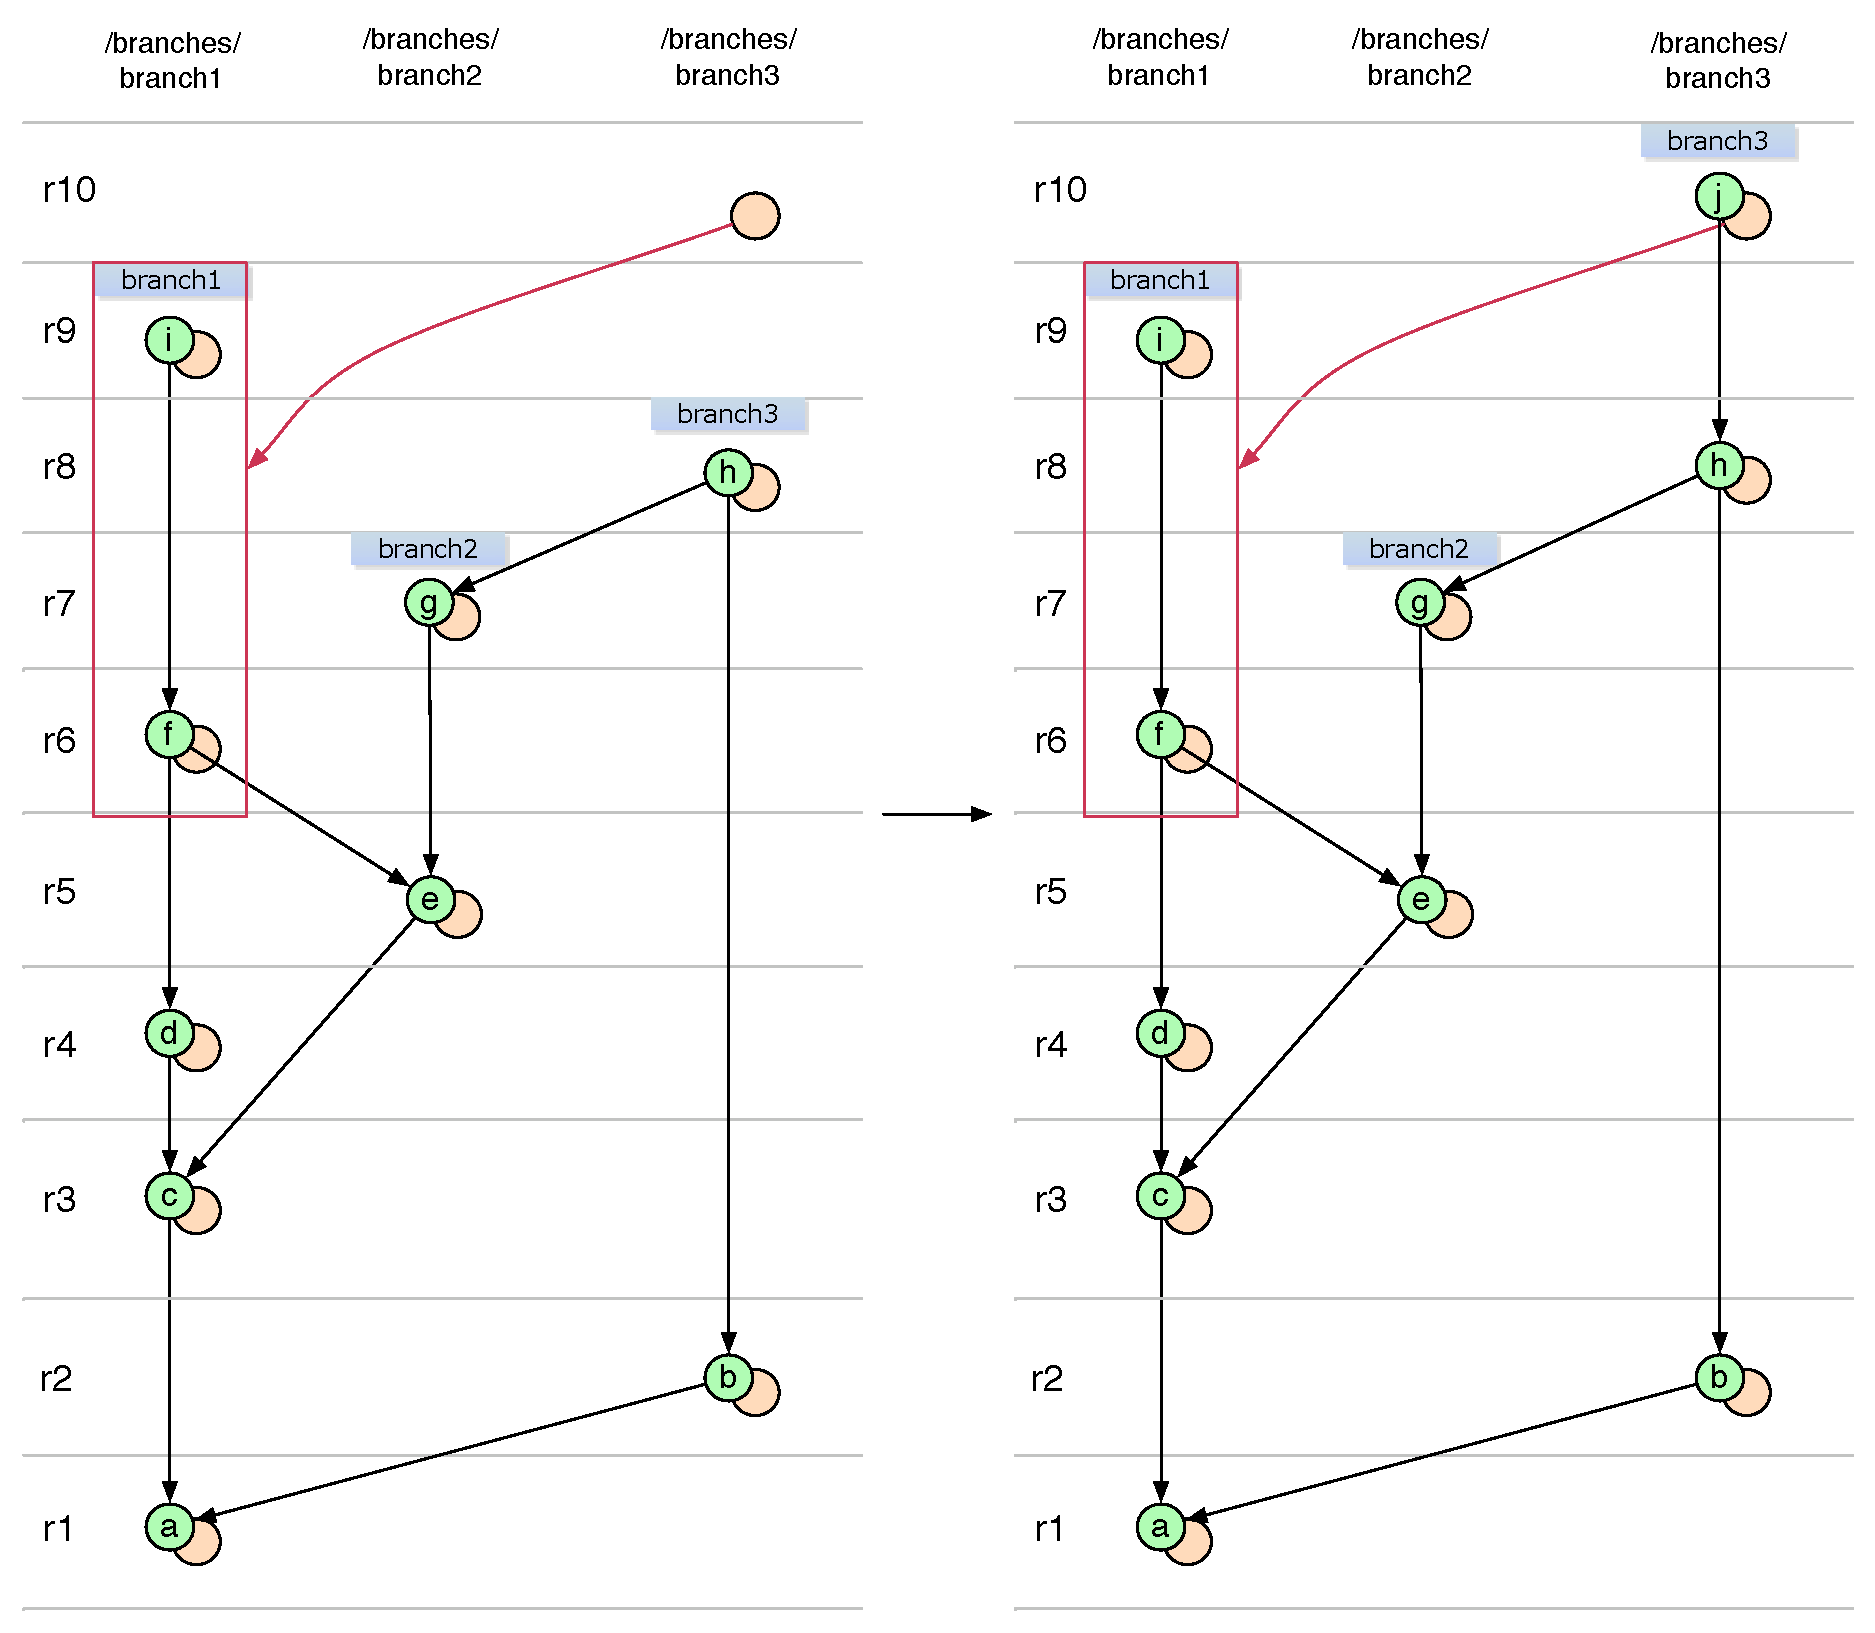
\includegraphics[width=\textwidth]{img/diagrams/no_merge_commit_cherry_pick_sequence_svn_to_git.pdf}%
\captionof{figure}{Merge of Git branch which is available from another branch being translated to a sequence of Subversion revisions.}
\label{no_merge_commit_cherry_pick_sequence_svn_to_git}%
\end{center}

\subsubsection{Octopus Merge}

\begin{center}
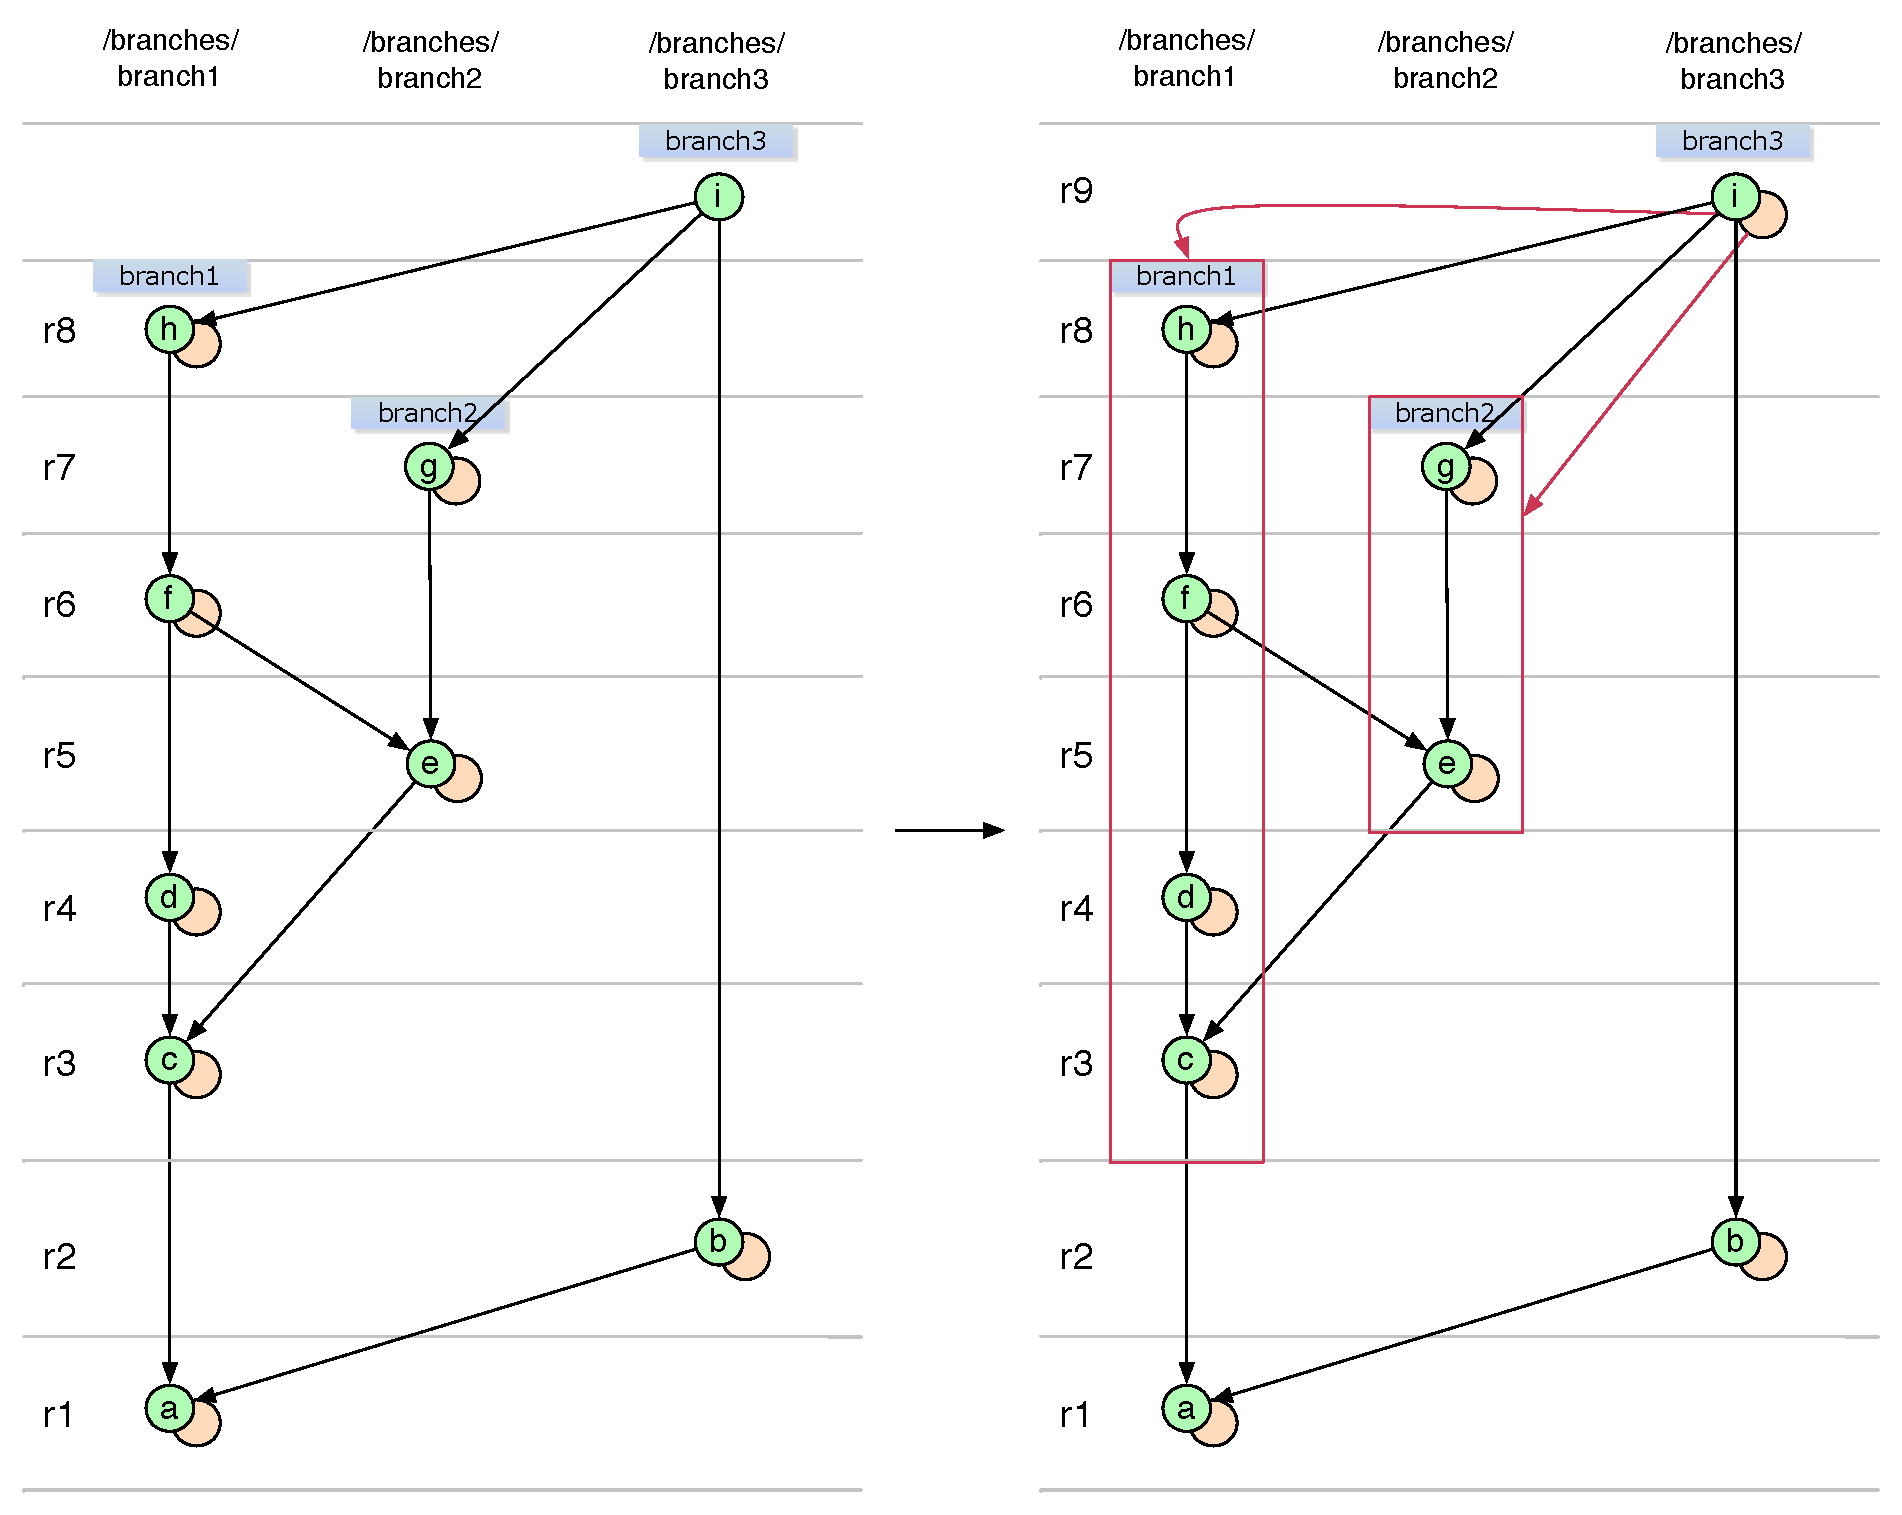
\includegraphics[width=\textwidth]{img/diagrams/octopus_merge_git_to_svn.pdf}%
\captionof{figure}{Octopus merge commit being translated to svn:mergeinfo change.}
\label{octopus_merge_git_to_svn}%
\end{center}

\begin{center}
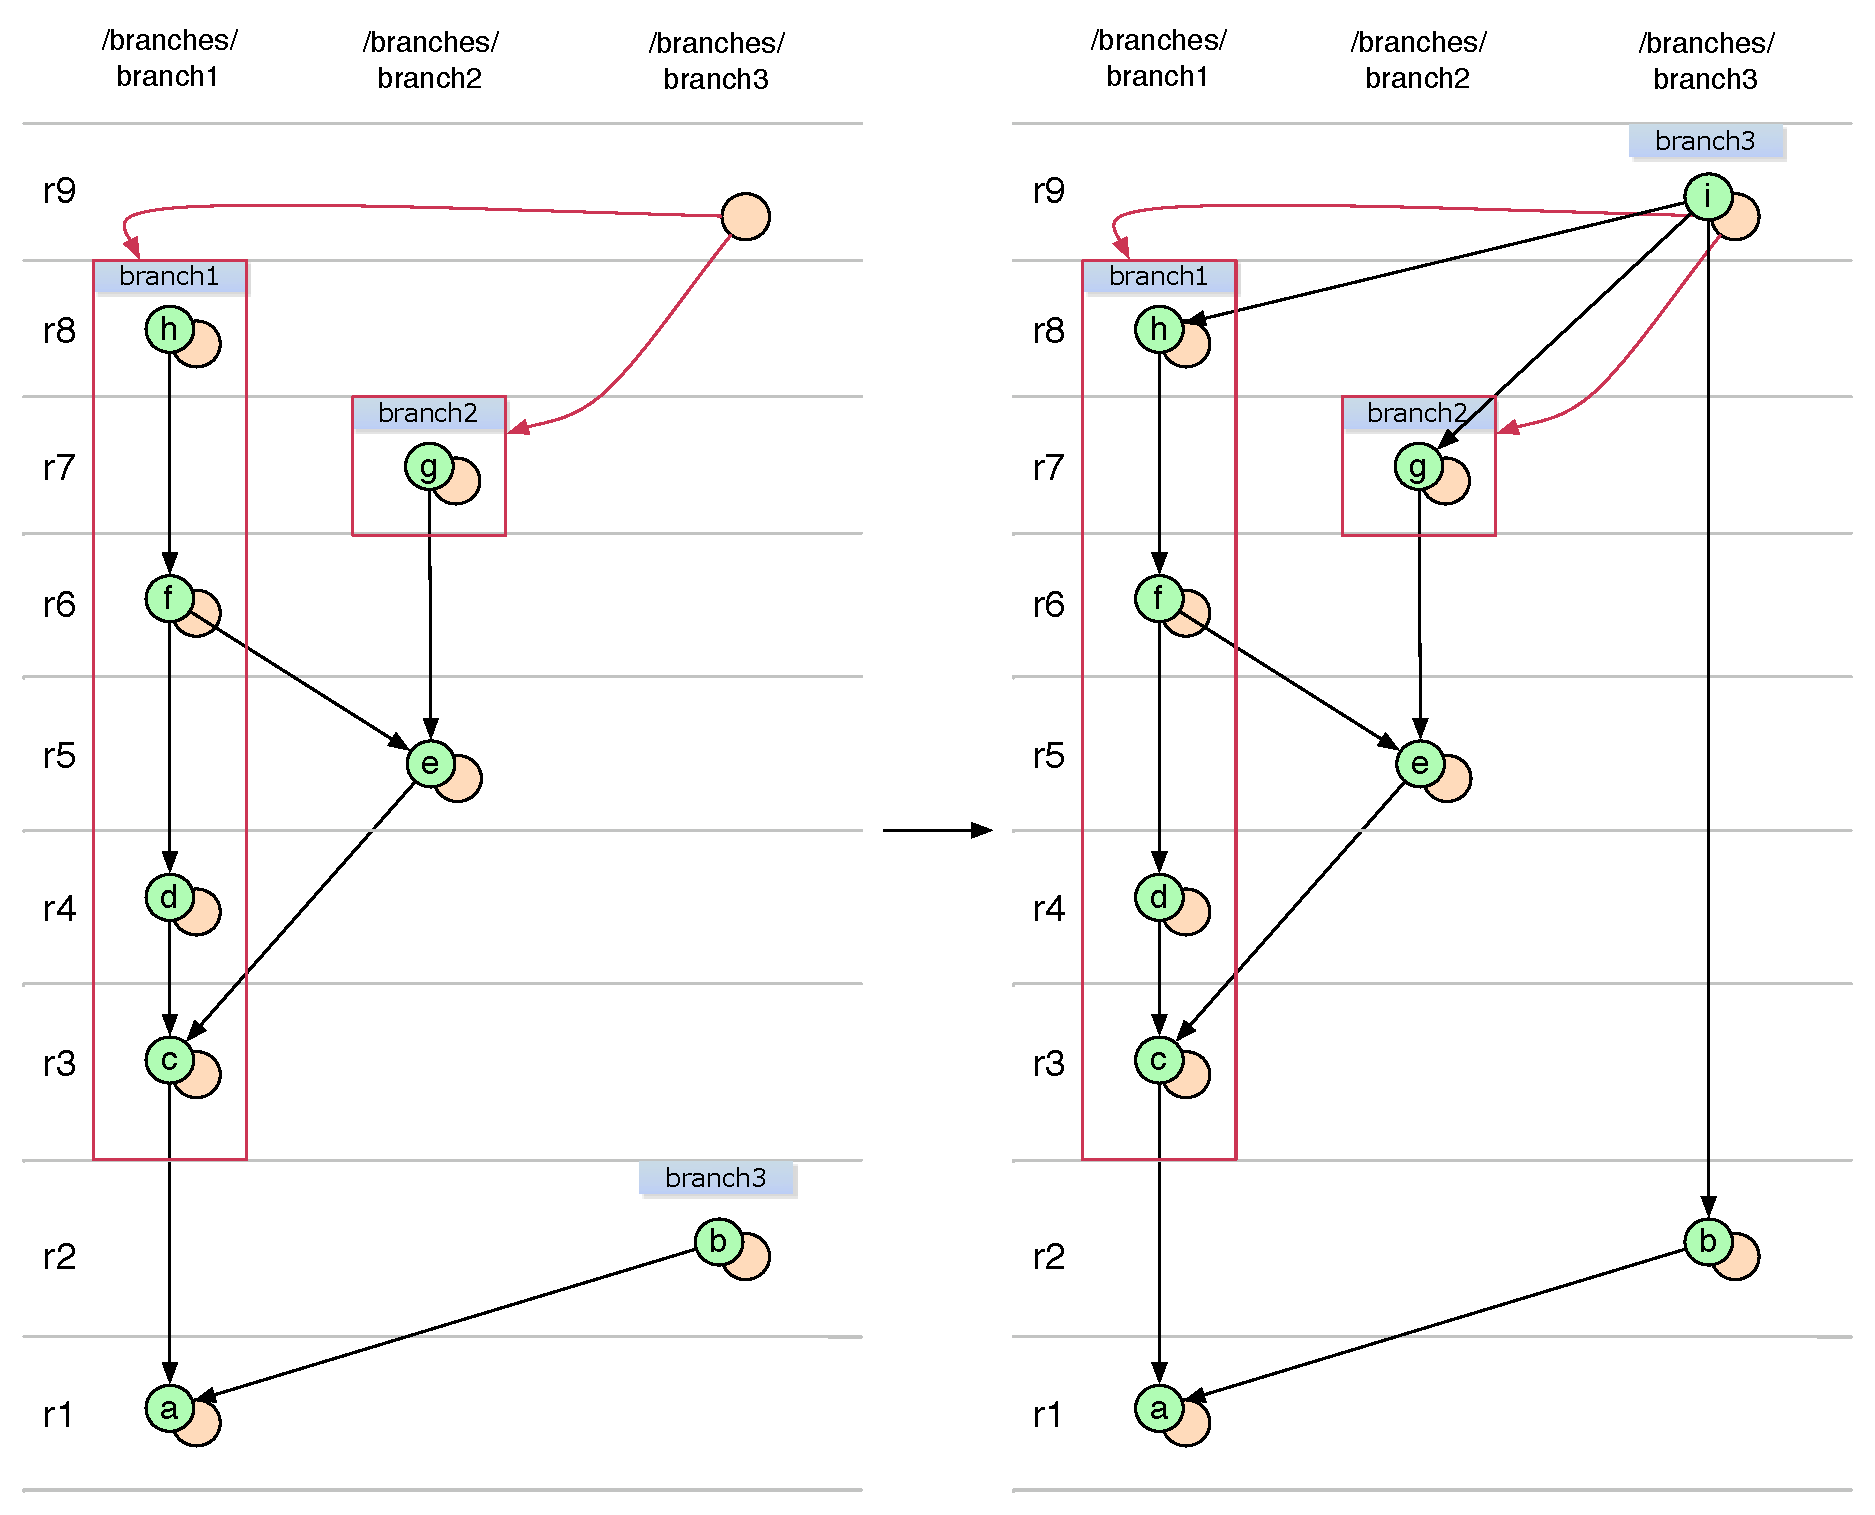
\includegraphics[width=\textwidth]{img/diagrams/octopus_merge_svn_to_git.pdf}%
\captionof{figure}{Change of svn:mergeinfo property being translated to octopus merge commit.}
\label{octopus_merge_svn_to_git}%
\end{center}
